\chapter{\RU{Примеры разбора закрытых (proprietary) форматов файлов}\EN{Examples of reversing proprietary file formats}\ESph{}\PTBRph{}\PLph{}\ITAph{}
\DE{Beispiele für das Reverse Engineering proprietärer Dateiformate}
\NLph{}}

% sections
\section{\RU{Примитивное XOR-шифрование}\EN{Primitive XOR-encryption}}
\label{simple_XOR_encryption}

\ifdefined\RUSSIAN
В русскоязычной литературе также используется термин \IT{гаммирование}.
\fi

% subsections
\EN{% TODO translate
\subsection{Simplest ever XOR encryption}

I once saw a software where all debugging messages has been encrypted using XOR by value of 3.
In other words, two lowest bits of all characters has been flipped.

``Hello, world'' would become ``Kfool/\#tlqog'':

\begin{lstlisting}
#!/usr/bin/python

msg="Hello, world!"

print "".join(map(lambda x: chr(ord(x)^3), msg))
\end{lstlisting}

This is quite interesting encryption (or rather obfuscation), because it has two important properties:
1) single function for encryption/decryption, just apply it again;
2) resulting characters are also printable, so the whole string can be used in source code without escaping characters.

The second property exploits the fact that all printable characters organized in rows: 0x2x-0x7x, and when you 
flip two lowest bits, character \IT{moving} 1 or 3 characters left or right, but never \IT{moved} to another (maybe
non-printable) row:

\begin{figure}[H]
\centering
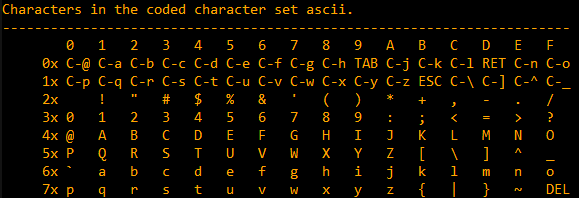
\includegraphics[width=0.7\textwidth]{ascii_clean.png}
\caption{7-bit \ac{ASCII} table in Emacs}
\end{figure}

\dots with a single exception of 0x7F character.

For example, let's \IT{encrypt} characters in A-Z range:

\begin{lstlisting}
#!/usr/bin/python

msg="@ABCDEFGHIJKLMNO"

print "".join(map(lambda x: chr(ord(x)^3), msg))
\end{lstlisting}

Result:
% FIXME \verb
\begin{lstlisting}
CBA@GFEDKJIHONML
\end{lstlisting}

It's like ``@'' and ``C'' characters has been swapped, and so are ``B'' and ``a''.

Yet again, this is interesting example of exploiting XOR properties, rather than encryption:
the very same effect of \IT{preserving printableness} can be achieved while flipping any of lowest 4 bits,
in any combination.

}
\EN{\clearpage
\subsection{Norton Guide: simplest possible 1-byte XOR encryption}
\label{norton_guide}

Norton Guide\footnote{\href{http://go.yurichev.com/17116}{wikipedia}} was popular in the epoch of MS-DOS, it was a resident program that worked as a hypertext reference manual.

Norton Guide's databases are files with the extension .ng, the contents of which look encrypted:

\begin{figure}[H]
\centering
\myincludegraphics{ff/XOR/ng/ng1.png}
\caption{Very typical look}
\end{figure}

Why did we think that it's encrypted but not compressed?

We see that the 0x1A byte (looking like \q{$\rightarrow$}) occurs often, it would not be possible in a compressed file.

We also see long parts that consist only of Latin letters, and they look like strings in an unknown
language.

\clearpage
Since the 0x1A byte occurs so often, we can try to decrypt the file, assuming that it's encrypted
by the simplest XOR-encryption.

If we apply XOR with the 0x1A constant to each byte in Hiew, we can see familiar English text strings:

\begin{figure}[H]
\centering
\myincludegraphics{ff/XOR/ng/ng2.png}
\caption{Hiew XORing with 0x1A}
\end{figure}

XOR encryption with one single constant byte is the simplest possible encryption method, which is, nevertheless,
encountered sometimes.

Now we understand why the 0x1A byte is occurring so often: because there are so many zero bytes and they
were replaced by 0x1A in encrypted form.

But the constant might be different.
In this case, we could try every constant in the 0..255 range and look for something familiar in the decrypted
file. 256 is not so much.

More about Norton Guide's file format: \url{http://go.yurichev.com/17317}.

\subsubsection{Entropy}
\myindex{Wolfram Mathematica}
\myindex{Entropy}

A very important property of such primitive encryption systems is that the information entropy
of the encrypted/decrypted block is the same.

Here is my analysis in Wolfram Mathematica 10.

\begin{lstlisting}[caption=Wolfram Mathematica 10,style=custommath]
In[1]:= input = BinaryReadList["X86.NG"];

In[2]:= Entropy[2, input] // N
Out[2]= 5.62724

In[3]:= decrypted = Map[BitXor[#, 16^^1A] &, input];

In[4]:= Export["X86_decrypted.NG", decrypted, "Binary"];

In[5]:= Entropy[2, decrypted] // N
Out[5]= 5.62724

In[6]:= Entropy[2, ExampleData[{"Text", "ShakespearesSonnets"}]] // N
Out[6]= 4.42366
\end{lstlisting}

What we do here is load the file, get its entropy, decrypt it, save it and get the entropy again (the same!).

Mathematica also offers some well-known English language texts for analysis.

So we also get the entropy of Shakespeare's sonnets, and it is close to the entropy of the file we just analyzed.

The file we analyzed consists of English language sentences, which are close to the language 
of Shakespeare.

And the XOR-ed bitwise English language text has the same entropy.

% I checked!
However, this is not true when the file is XOR-ed with a pattern larger than one byte.

The file we analyzed can be downloaded here: \url{http://go.yurichev.com/17350}.

\myparagraph{One more word about base of entropy}

\newcommand{\FNENTURL}{\footnote{\url{http://www.fourmilab.ch/random/}}}

Wolfram Mathematica calculates entropy with base of $e$ (base of the natural logarithm),
and the UNIX \IT{ent} utility\FNENTURL uses base 2.

So we set base 2 explicitly in \TT{Entropy} command, so Mathematica will give us the same results as the \IT{ent} utility.

}\RU{\clearpage
\subsection{Norton Guide: простейшее однобайтное XOR-шифрование}
\label{norton_guide}

Norton Guide\footnote{\href{http://go.yurichev.com/17116}{wikipedia}} был популярен во времена MS-DOS, это была резидентная программа, работающая как
гипертекстовый справочник.

Базы данных Norton Guide это файлы с расширением .ng, содержимое которых выглядит как зашифрованное:

\begin{figure}[H]
\centering
\myincludegraphics{ff/XOR/ng/ng1.png}
\caption{Очень типичный вид}
\end{figure}

Почему мы думаем, что зашифрованное а не сжатое? 

Мы видим, как слишком часто попадается байт 0x1A (который выглядит как \q{$\rightarrow$}), в сжатом файле такого не было бы никогда.

Во-вторых, мы видим длинные части состоящие только из латинских букв, они выглядят как строки
на незнакомом языке.

\clearpage

Из-за того, что байт 0x1A слишком часто встречается, мы можем попробовать расшифровать файл, полагая
что он зашифрован простейшим XOR-шифрованием.

Применяем XOR с константой 0x1A к каждому байту в Hiew и мы можем видеть знакомые текстовые строки на английском:

\begin{figure}[H]
\centering
\myincludegraphics{ff/XOR/ng/ng2.png}
\caption{Hiew применение XOR с 0x1A}
\end{figure}

XOR-шифрование с одним константным байтом это самый простой способ шифрования, который, тем не менее, иногда
встречается.

Теперь понятно почему байт 0x1A так часто встречался: потому что в файле очень много нулевых байт 
и в зашифрованном виде они везде были заменены на 0x1A.

Но эта константа могла быть другой.

В таком случае, можно было бы попробовать перебрать все 256 комбинаций, и посмотреть содержимое \q{на глаз}, 
а 256 --- это совсем немного.

Больше о формате файлов Norton Guide: \url{http://go.yurichev.com/17317}.

\subsubsection{Энтропия}
\myindex{Wolfram Mathematica}
\myindex{Энтропия}

Очень важное свойство подобного примитивного шифрования в том, что информационная энтропия
зашифрованного/дешифрованного блока точно такая же.
Вот мой анализ в Wolfram Mathematica 10.

\begin{lstlisting}[caption=Wolfram Mathematica 10,style=custommath]
In[1]:= input = BinaryReadList["X86.NG"];

In[2]:= Entropy[2, input] // N
Out[2]= 5.62724

In[3]:= decrypted = Map[BitXor[#, 16^^1A] &, input];

In[4]:= Export["X86_decrypted.NG", decrypted, "Binary"];

In[5]:= Entropy[2, decrypted] // N
Out[5]= 5.62724

In[6]:= Entropy[2, ExampleData[{"Text", "ShakespearesSonnets"}]] // N
Out[6]= 4.42366
\end{lstlisting}

Что мы здесь делаем это загружаем файл, вычисляем его энтропию, дешифруем его, сохраняем, снова вычисляем энтропию (точно такая же!).

Mathematica дает возможность анализировать некоторые хорошо известные англоязычные тексты.

Так что мы вычисляем энтропию сонетов Шейкспира, и она близка к энтропии анализируемого нами файла.

Анализируемый нами файл состоит из предложений на английском языке, которые близки к языку
Шейкспира.

И применение побайтового XOR к тексту на английском языке не меняет энтропию.

% I checked!

Хотя, это не будет справедливо когда файл зашифрован при помощи XOR шаблоном длиннее одного байта.

Файл, который мы анализировали, можно скачать здесь: \url{http://go.yurichev.com/17350}.

\myparagraph{Еще кое-что о базе энтропии}

\newcommand{\FNENTURL}{\footnote{\url{http://www.fourmilab.ch/random/}}}

Wolfram Mathematica вычисляет энтропию с базой $e$ (основание натурального логарифма),
а утилита UNIX \IT{ent}\FNENTURL использует базу 2.

Так что мы явно указываем базу 2 в команде \TT{Entropy}, чтобы Mathematica давала те же результаты, что и утилита \IT{ent}.
}
\EN{\section{Network address calculation example}

As we know, a TCP/IP address (IPv4) consists of four numbers in the $0 \ldots 255$ range, i.e., four bytes.

Four bytes can be fit in a 32-bit variable easily, so an IPv4 host address, network mask or network address
can all be 32-bit integers.

From the user's point of view, the network mask is defined as four numbers and is formatted like 255.255.255.0 or so,
but network engineers (sysadmins) use a more compact notation (\ac{CIDR}), like \q{/8}, \q{/16}, etc.

This notation just defines the number of bits the mask has, starting at the \ac{MSB}.

\small
\begin{center}
\begin{tabular}{ | l | l | l | l | l | l | }
\hline
\HeaderColor Mask & 
\HeaderColor Hosts & 
\HeaderColor Usable &
\HeaderColor Netmask &
\HeaderColor Hex mask &
\HeaderColor \\
\hline
/30  & 4        & 2        & 255.255.255.252  & 0xfffffffc  & \\
\hline
/29  & 8        & 6        & 255.255.255.248  & 0xfffffff8  & \\
\hline
/28  & 16       & 14       & 255.255.255.240  & 0xfffffff0  & \\
\hline
/27  & 32       & 30       & 255.255.255.224  & 0xffffffe0  & \\
\hline
/26  & 64       & 62       & 255.255.255.192  & 0xffffffc0  & \\
\hline
/24  & 256      & 254      & 255.255.255.0    & 0xffffff00  & class C network \\
\hline
/23  & 512      & 510      & 255.255.254.0    & 0xfffffe00  & \\
\hline
/22  & 1024     & 1022     & 255.255.252.0    & 0xfffffc00  & \\
\hline
/21  & 2048     & 2046     & 255.255.248.0    & 0xfffff800  & \\
\hline
/20  & 4096     & 4094     & 255.255.240.0    & 0xfffff000  & \\
\hline
/19  & 8192     & 8190     & 255.255.224.0    & 0xffffe000  & \\
\hline
/18  & 16384    & 16382    & 255.255.192.0    & 0xffffc000  & \\
\hline
/17  & 32768    & 32766    & 255.255.128.0    & 0xffff8000  & \\
\hline
/16  & 65536    & 65534    & 255.255.0.0      & 0xffff0000  & class B network \\
\hline
/8   & 16777216 & 16777214 & 255.0.0.0        & 0xff000000  & class A network \\
\hline
\end{tabular}
\end{center}
\normalsize

Here is a small example, which calculates the network address by applying the network mask to the host address.

\lstinputlisting{\CURPATH/netmask.c}

\subsection{calc\_network\_address()}

\TT{calc\_network\_address()} function is simplest one: 
it just ANDs the host address with the network mask, resulting in the network address.

\lstinputlisting[caption=\Optimizing MSVC 2012 /Ob0,numbers=left]{\CURPATH/calc_network_address_MSVC_2012_Ox.asm}

At line 22 we see the most important \AND---here the network address is calculated.

\subsection{form\_IP()}

The \TT{form\_IP()} function just puts all 4 bytes into a 32-bit value.

Here is how it is usually done:

\begin{itemize}
\item Allocate a variable for the return value.  Set it to 0.

\item Take the fourth (lowest) byte, apply OR operation to this byte and return the value.
The return value contain the 4th byte now.

\item Take the third byte, shift it left by 8 bits.
You'll get a value like \TT{0x0000bb00} where \TT{bb} is your third byte.
Apply the OR operation to the resulting value and it.
The return value has contained \TT{0x000000aa} so far, so ORing the values will produce a value 
like \TT{0x0000bbaa}.

\item Take the second byte, shift it left by 16 bits.
You'll get a value like \TT{0x00cc0000}, where \TT{cc} is your second byte.
Apply the OR operation to the resulting value and return it.
The return value has contained \TT{0x0000bbaa} so far, so ORing the values will produce
a value like \TT{0x00ccbbaa}.

\item Take the first byte, shift it left by 24 bits.
You'll get a value like \TT{0xdd000000}, where \TT{dd} is your first byte.
Apply the OR operation to the resulting value and return it.
The return value contain \TT{0x00ccbbaa} so far, so ORing the values will produce
a value like \TT{0xddccbbaa}.

\end{itemize}

And this is how it's done by non-optimizing MSVC 2012:

\lstinputlisting[caption=\NonOptimizing MSVC 2012]{\CURPATH/form_IP_MSVC_2012_EN.asm}

Well, the order is different, but, of course, the order of the operations doesn't matter.

\Optimizing MSVC 2012 does essentially the same, but in a different way:

\lstinputlisting[caption=\Optimizing MSVC 2012 /Ob0]{\CURPATH/form_IP_MSVC_2012_Ox_EN.asm}

We could say that each byte is written to the lowest 8 bits of the return value, 
and then the return value is shifted left by one byte at each step.

Repeat 4 times for each input byte.

\par
That's it! Unfortunately, there are probably no other ways to do it.

There are no popular \ac{CPU}s or \ac{ISA}s which has instruction for composing a value from
bits or bytes.

It's all usually done by bit shifting and ORing.

\subsection{print\_as\_IP()}

\TT{print\_as\_IP()} does the inverse: splitting a 32-bit value into 4 bytes.

Slicing works somewhat simpler: just shift input value by 24, 16, 8 or 0 bits, take the 
bits from zeroth to seventh (lowest byte), and that's it:

\lstinputlisting[caption=\NonOptimizing MSVC 2012]{\CURPATH/print_as_IP_MSVC_2012_EN.asm}

\Optimizing MSVC 2012 does almost the same, but without unnecessary reloading of the input value:

\lstinputlisting[caption=\Optimizing MSVC 2012 /Ob0]{\CURPATH/print_as_IP_MSVC_2012_Ox.asm}

\subsection{form\_netmask() and set\_bit()}

\TT{form\_netmask()} makes a network mask value from \ac{CIDR} notation.
Of course, it would be much effective to use here some kind of a precalculated table, but we consider it in this
way intentionally, to demonstrate bit shifts.

We will also write a separate function \TT{set\_bit()}. 
It's a not very good idea to create a function
for such primitive operation, but it would be easy to understand how it all works.

\lstinputlisting[caption=\Optimizing MSVC 2012 /Ob0]{\CURPATH/form_netmask_MSVC_2012_Ox.asm}

\TT{set\_bit()} is primitive: it just shift left 1 to number of bits we need and then 
ORs it with the \q{input} value.
\TT{form\_netmask()} has a loop: it will set as many bits (starting from the \ac{MSB}) as 
passed in the \TT{netmask\_bits} argument

\subsection{Summary}

That's it!
We run it and getting:

\begin{lstlisting}
netmask=255.255.255.0
network address=10.1.2.0
netmask=255.0.0.0
network address=10.0.0.0
netmask=255.255.255.128
network address=10.1.2.0
netmask=255.255.255.192
network address=10.1.2.64
\end{lstlisting}
}\RU{\myparagraph{\NonOptimizing MSVC}

Вот что выдал MSVC 2010:

\lstinputlisting[caption=\NonOptimizing MSVC 2010,style=customasm]{patterns/12_FPU/3_comparison/x86/MSVC/MSVC_RU.asm}

\myindex{x86!\Instructions!FLD}
Итак, \FLD загружает \GTT{\_b} в регистр \ST{0}.

\label{Czero_etc}
\newcommand{\Czero}{\GTT{C0}\xspace}
\newcommand{\Ctwo}{\GTT{C2}\xspace}
\newcommand{\Cthree}{\GTT{C3}\xspace}
\newcommand{\CThreeBits}{\Cthree/\Ctwo/\Czero}

\myindex{x86!\Instructions!FCOMP}
\FCOMP сравнивает содержимое \ST{0} с тем, что лежит в \GTT{\_a} и выставляет биты \CThreeBits в 
регистре статуса FPU. Это 16-битный регистр отражающий текущее состояние FPU.

После этого инструкция \FCOMP также выдергивает одно значение из стека. 
Это отличает её от \FCOM, которая просто сравнивает значения, оставляя стек в таком же состоянии.

К сожалению, у процессоров до Intel P6
\footnote{Intel P6 это Pentium Pro, Pentium II, и последующие модели} нет инструкций условного перехода,
проверяющих биты \CThreeBits.
Возможно, так сложилось исторически (вспомните о том, что FPU когда-то был вообще отдельным чипом).\\
А у Intel P6 появились инструкции \FCOMI/\FCOMIP/\FUCOMI/\FUCOMIP, делающие то же самое, 
только напрямую модифицирующие флаги \ZF/\PF/\CF.

\myindex{x86!\Instructions!FNSTSW}
Так что \FNSTSW копирует содержимое регистра статуса в \AX. 
Биты \CThreeBits занимают позиции, 
соответственно, 14, 10, 8. В этих позициях они и остаются в регистре \AX, 
и все они расположены в старшей части регистра~--- \AH.

\begin{itemize}
\item Если $b>a$ в нашем случае, то биты \CThreeBits должны быть выставлены так: 0, 0, 0.
\item Если $a>b$, то биты будут выставлены: 0, 0, 1.
\item Если $a=b$, то биты будут выставлены так: 1, 0, 0.
\item Если результат не определен (в случае ошибки), то биты будут выставлены так: 1, 1, 1.
\end{itemize}
% TODO: table here?

Вот как биты \CThreeBits расположены в регистре \AX:

\begin{center}
\begin{bytefield}[endianness=big,bitwidth=0.03\linewidth]{16}
\bitheader{14,10,9,8} \\
\bitbox{1}{} & 
\bitbox{1}{C3} & 
\bitbox{3}{} & 
\bitbox{1}{C2} & 
\bitbox{1}{C1} & 
\bitbox{1}{C0} &
\bitbox{8}{}
\end{bytefield}
\end{center}


Вот как биты \CThreeBits расположены в регистре \AH:

\begin{center}
\begin{bytefield}[endianness=big,bitwidth=0.03\linewidth]{8}
\bitheader{6,2,1,0} \\
\bitbox{1}{} & 
\bitbox{1}{C3} & 
\bitbox{3}{} & 
\bitbox{1}{C2} & 
\bitbox{1}{C1} & 
\bitbox{1}{C0}
\end{bytefield}
\end{center}


После исполнения \INS{test ah, 5}\footnote{5=101b} % FIXME: subscript here!
будут учтены только биты \Czero и \Ctwo (на позициях 0 и 2), остальные просто проигнорированы.

\label{parity_flag}
\myindex{x86!\Registers!\Flags!Флаг четности}
Теперь немного о \IT{parity flag}\footnote{флаг четности}. 
Ещё один замечательный рудимент эпохи.

Этот флаг выставляется в 1 если количество единиц в последнем результате четно. 
И в 0 если нечетно.

Заглянем в Wikipedia\footnote{\href{http://go.yurichev.com/17131}{wikipedia.org/wiki/Parity\_flag}}:

\begin{framed}
\begin{quotation}
One common reason to test the parity flag actually has nothing to do with parity. The FPU has four condition flags 
(C0 to C3), but they cannot be tested directly, and must instead be first copied to the flags register. 
When this happens, C0 is placed in the carry flag, C2 in the parity flag and C3 in the zero flag. 
The C2 flag is set when e.g. incomparable floating point values (NaN or unsupported format) are compared 
with the FUCOM instructions.
\end{quotation}
\end{framed}

Как упоминается в Wikipedia, флаг четности иногда используется в FPU-коде и сейчас мы увидим как.

\myindex{x86!\Instructions!JP}
Флаг \PF будет выставлен в 1, если \Czero и \Ctwo оба 1 или оба 0. 
И тогда сработает последующий \JP (\IT{jump if PF==1}). 
Если мы вернемся чуть назад и посмотрим значения \CThreeBits 
для разных вариантов, то увидим, что условный переход \JP сработает в двух случаях: если $b>a$ или если $a=b$ 
(ведь бит \Cthree перестал учитываться после исполнения \INS{test ah, 5}).

Дальше всё просто. Если условный переход сработал, то \FLD загрузит значение \INS{\_b} в \ST{0}, 
а если не сработал, то загрузится \GTT{\_a} и произойдет выход из функции.

\mysubparagraph{А как же проверка флага \Ctwo?}

Флаг \Ctwo включается в случае ошибки (\gls{NaN}, итд.), но наш код его не проверяет.

Если программисту нужно знать, не произошла ли FPU-ошибка, он должен позаботиться об этом
дополнительно, добавив соответствующие проверки.

\clearpage
\mysubparagraph{\olly}
\myindex{\olly}

Попробуем этот пример в \olly.
Входное значение функции (2) загружается в \EAX: 

\begin{figure}[H]
\centering
\myincludegraphics{patterns/08_switch/2_lot/olly1.png}
\caption{\olly: входное значение функции загружено в \EAX}
\label{fig:switch_lot_olly1}
\end{figure}

\clearpage
Входное значение проверяется, не больше ли оно чем 4? 
Нет, переход по умолчанию (\q{default}) не будет исполнен:

\begin{figure}[H]
\centering
\myincludegraphics{patterns/08_switch/2_lot/olly2.png}
\caption{\olly: 2 не больше чем 4: переход не сработает}
\label{fig:switch_lot_olly2}
\end{figure}

\clearpage
Здесь мы видим jumptable:

\begin{figure}[H]
\centering
\myincludegraphics{patterns/08_switch/2_lot/olly3.png}
\caption{\olly: вычисляем адрес для перехода используя jumptable}
\label{fig:switch_lot_olly3}
\end{figure}

Кстати, щелкнем по \q{Follow in Dump} $\rightarrow$ \q{Address constant}, так что теперь \IT{jumptable} видна в окне данных.

Это 5 32-битных значений\footnote{Они подчеркнуты в \olly, потому что это также и FIXUP-ы: \myref{subsec:relocs}, мы вернемся к ним позже}.
\ECX сейчас содержит 2, так что третий элемент (либо второй, если считать с нулевого) таблицы будет использован.
Кстати, можно также щелкнуть \q{Follow in Dump} $\rightarrow$ \q{Memory address} и \olly покажет элемент, который сейчас адресуется в инструкции \JMP. 
Это \TT{0x010B103A}.

\clearpage
Переход сработал и мы теперь на \TT{0x010B103A}: сейчас будет исполнен код, выводящий строку \q{two}:

\begin{figure}[H]
\centering
\myincludegraphics{patterns/08_switch/2_lot/olly4.png}
\caption{\olly: теперь мы на соответствующей метке \IT{case:}}
\label{fig:switch_lot_olly4}
\end{figure}

}
\EN{% TODO translate
\subsection{Simple encryption using XOR mask}
\label{XOR_mask_1}

I've found an old interactive fiction game while diving deep into \IT{if-archive}\footnote{\url{http://www.ifarchive.org/}}:

\begin{lstlisting}
The New Castle v3.5 - Text/Adventure Game
in the style of the original Infocom (tm)
type games, Zork, Collosal Cave (Adventure),
etc.  Can you solve the mystery of the
abandoned castle?
Shareware from Software Customization.
Software Customization [ASP] Version 3.5 Feb. 2000
\end{lstlisting}

It's downloadable here: \url{http://yurichev.com/blog/XOR_mask_1/files/newcastle.tgz}.

There is a file inside (named \IT{castle.dbf}) which is clearly encrypted, but not by a real crypto algorithm, nor it's compressed, this is something rather simpler.
I wouldn't even measure entropy level (\myref{entropy}) of the file.
Here is how it looks like in Midnight Commander:

\begin{figure}[H]
\centering
\myincludegraphics{ff/XOR/mask_1/mc_encrypted.png}
\caption{Encrypted file in Midnight Commander}
\end{figure}

The encrypted file can be downloaded \href{http://yurichev.com/blog/XOR_mask_1/files/castle.dbf}{here}.

Will it be possible to decrypt it without accessing to the program, using just this file?

There is a clearly visible pattern of repeating string.
If a simple encryption by XOR mask was applied, such repeating strings is a prominent signature, because, probably, there were a long lacunas of zero bytes,
which, in turn, are present in many executable files as well as in binary data files.

\myindex{UNIX!xxd}
Here I'll dump the file's beginning using \IT{xxd} UNIX utility:

\lstinputlisting{ff/XOR/mask_1/xxd_result.txt}

Let's stick at visible repeating \q{iubgv} string.
By looking at this dump, we can clearly see that the period of the string occurrence is 0x51 or 81.
Probably, 81 is size of block?
Size of the file is 1658961, and it can be divided evenly by 81 (and there are 20481 blocks then).

Now I'll use Mathematica to analyze, are there repeating 81-byte blocks in the file?
I'll split input file by 81-byte blocks and then I'll use 
\IT{Tally[]}\footnote{\url{https://reference.wolfram.com/language/ref/Tally.html}}
function which just calculates, how many times some item has been occurred in the input list.
Tally's output is not sorted, so I also add \IT{Sort[]} function to sort it by number of occurrences in descending order.

\begin{lstlisting}[style=custommath]
input = BinaryReadList["/home/dennis/.../castle.dbf"];

blocks = Partition[input, 81];

stat = Sort[Tally[blocks], #1[[2]] > #2[[2]] &]
\end{lstlisting}

And here is output:

\begin{lstlisting}[style=custommath]
{{{80, 103, 2, 116, 113, 102, 118, 25, 99, 8, 19, 23, 116, 125, 107, 
   25, 99, 109, 114, 102, 14, 121, 115, 31, 9, 117, 113, 111, 5, 4, 
   127, 28, 122, 101, 8, 110, 14, 18, 124, 106, 16, 20, 104, 119, 8, 
   109, 26, 106, 9, 97, 13, 99, 15, 119, 20, 105, 117, 98, 103, 118, 
   1, 126, 29, 97, 122, 17, 15, 114, 110, 3, 5, 125, 125, 99, 126, 
   119, 102, 30, 122, 2, 117}, 1739}, 
{{80, 100, 2, 116, 113, 102, 118, 25, 99, 8, 19, 23, 116, 
   125, 107, 25, 99, 109, 114, 102, 14, 121, 115, 31, 9, 117, 113, 
   111, 5, 4, 127, 28, 122, 101, 8, 110, 14, 18, 124, 106, 16, 20, 
   104, 119, 8, 109, 26, 106, 9, 97, 13, 99, 15, 119, 20, 105, 117, 
   98, 103, 118, 1, 126, 29, 97, 122, 17, 15, 114, 110, 3, 5, 125, 
   125, 99, 126, 119, 102, 30, 122, 2, 117}, 1422}, 
{{80, 101, 2, 116, 113, 102, 118, 25, 99, 8, 19, 23, 116, 
   125, 107, 25, 99, 109, 114, 102, 14, 121, 115, 31, 9, 117, 113, 
   111, 5, 4, 127, 28, 122, 101, 8, 110, 14, 18, 124, 106, 16, 20, 
   104, 119, 8, 109, 26, 106, 9, 97, 13, 99, 15, 119, 20, 105, 117, 
   98, 103, 118, 1, 126, 29, 97, 122, 17, 15, 114, 110, 3, 5, 125, 
   125, 99, 126, 119, 102, 30, 122, 2, 117}, 1012},
{{80, 120, 2, 116, 113, 102, 118, 25, 99, 8, 19, 23, 116, 
   125, 107, 25, 99, 109, 114, 102, 14, 121, 115, 31, 9, 117, 113, 
   111, 5, 4, 127, 28, 122, 101, 8, 110, 14, 18, 124, 106, 16, 20, 
   104, 119, 8, 109, 26, 106, 9, 97, 13, 99, 15, 119, 20, 105, 117, 
   98, 103, 118, 1, 126, 29, 97, 122, 17, 15, 114, 110, 3, 5, 125, 
   125, 99, 126, 119, 102, 30, 122, 2, 117}, 377},

...

{{80, 2, 74, 49, 113, 21, 62, 88, 39, 71, 68, 23, 63, 51, 36, 78, 48, 
   108, 114, 102, 14, 121, 115, 31, 9, 117, 113, 111, 5, 4, 127, 28, 
   122, 101, 8, 110, 14, 18, 124, 106, 16, 20, 104, 119, 8, 109, 26, 
   106, 9, 97, 13, 99, 15, 119, 20, 105, 117, 98, 103, 118, 1, 126, 
   29, 97, 122, 17, 15, 114, 110, 3, 5, 125, 125, 99, 126, 119, 102, 
   30, 122, 2, 117}, 1},
{{80, 1, 74, 59, 113, 45, 56, 86, 52, 91, 19, 64, 60, 60, 63, 
   25, 38, 59, 59, 42, 14, 53, 38, 77, 66, 38, 113, 38, 75, 4, 43, 84,
    63, 101, 64, 43, 79, 64, 40, 57, 16, 91, 46, 119, 69, 40, 84, 117,
    9, 97, 13, 99, 15, 119, 20, 105, 117, 98, 103, 118, 1, 126, 29, 
   97, 122, 17, 15, 114, 110, 3, 5, 125, 125, 99, 126, 119, 102, 30, 
   122, 2, 117}, 1},
{{80, 2, 74, 49, 113, 49, 51, 92, 39, 8, 92, 81, 116, 62, 57, 
   80, 46, 40, 114, 36, 75, 56, 33, 76, 9, 55, 56, 59, 81, 65, 45, 28,
    60, 55, 93, 39, 90, 28, 124, 106, 16, 20, 104, 119, 8, 109, 26, 
   106, 9, 97, 13, 99, 15, 119, 20, 105, 117, 98, 103, 118, 1, 126, 
   29, 97, 122, 17, 15, 114, 110, 3, 5, 125, 125, 99, 126, 119, 102, 
   30, 122, 2, 117}, 1}}
\end{lstlisting}

Tally's output is list pairs, each pair has 81-byte block and number of times it has been occurred in the file.
We see that the most frequent block is the first, it has been occurred 1739 times.
The second one has been occurred 1422 times. There are others: 1012 times, 377 times, etc.
81-byte blocks which has been occurred just once are at the end of output.

Let's try to compare these blocks? The first and the second?
Is there a function in Mathematica which compares lists/arrays? Certainly is, but for educational purposes, I'll use XOR operation for comparison.
Indeed: if bytes in two input arrays are identical, XOR result is 0. If they are non-equal, result will be non-zero.

Let's compare first block (occurred 1739 times) and the second (occurred 1422 times):

\begin{lstlisting}[style=custommath]
In[]:= BitXor[stat[[1]][[1]], stat[[2]][[1]]]
Out[]= {0, 3, 0, 0, 0, 0, 0, 0, 0, 0, 0, 0, 0, 0, 0, 0, 0, 0, 0, \
0, 0, 0, 0, 0, 0, 0, 0, 0, 0, 0, 0, 0, 0, 0, 0, 0, 0, 0, 0, 0, 0, 0, \
0, 0, 0, 0, 0, 0, 0, 0, 0, 0, 0, 0, 0, 0, 0, 0, 0, 0, 0, 0, 0, 0, 0, \
0, 0, 0, 0, 0, 0, 0, 0, 0, 0, 0, 0, 0, 0, 0, 0}
\end{lstlisting}

They are differ only in the second byte.

Let's compare second (occurred 1422 times) and third (occurred 1012 times):

\begin{lstlisting}[style=custommath]
In[]:= BitXor[stat[[2]][[1]], stat[[3]][[1]]]
Out[]= {0, 1, 0, 0, 0, 0, 0, 0, 0, 0, 0, 0, 0, 0, 0, 0, 0, 0, 0, \
0, 0, 0, 0, 0, 0, 0, 0, 0, 0, 0, 0, 0, 0, 0, 0, 0, 0, 0, 0, 0, 0, 0, \
0, 0, 0, 0, 0, 0, 0, 0, 0, 0, 0, 0, 0, 0, 0, 0, 0, 0, 0, 0, 0, 0, 0, \
0, 0, 0, 0, 0, 0, 0, 0, 0, 0, 0, 0, 0, 0, 0, 0}
\end{lstlisting}

They are also differ only in the second byte.

Anyway, let's try to use the most occurred block as a XOR key and try to decrypt four first 81-byte blocks in the file:

\begin{lstlisting}[style=custommath]
In[]:= key = stat[[1]][[1]]
Out[]= {80, 103, 2, 116, 113, 102, 118, 25, 99, 8, 19, 23, 116, \
125, 107, 25, 99, 109, 114, 102, 14, 121, 115, 31, 9, 117, 113, 111, \
5, 4, 127, 28, 122, 101, 8, 110, 14, 18, 124, 106, 16, 20, 104, 119, \
8, 109, 26, 106, 9, 97, 13, 99, 15, 119, 20, 105, 117, 98, 103, 118, \
1, 126, 29, 97, 122, 17, 15, 114, 110, 3, 5, 125, 125, 99, 126, 119, \
102, 30, 122, 2, 117}

In[]:= ToASCII[val_] := If[val == 0, " ", FromCharacterCode[val, "PrintableASCII"]]

In[]:= DecryptBlockASCII[blk_] := Map[ToASCII[#] &, BitXor[key, blk]]

In[]:= DecryptBlockASCII[blocks[[1]]]
Out[]= {" ", " ", " ", " ", " ", " ", " ", " ", " ", " ", " ", " \
", " ", " ", " ", " ", " ", " ", " ", " ", " ", " ", " ", " ", " ", " \
", " ", " ", " ", " ", " ", " ", " ", " ", " ", " ", " ", " ", " ", " \
", " ", " ", " ", " ", " ", " ", " ", " ", " ", " ", " ", " ", " ", " \
", " ", " ", " ", " ", " ", " ", " ", " ", " ", " ", " ", " ", " ", " \
", " ", " ", " ", " ", " ", " ", " ", " ", " ", " ", " ", " ", " "}

In[]:= DecryptBlockASCII[blocks[[2]]]
Out[]= {" ", "e", "H", "E", " ", "W", "E", "E", "D", " ", "O", \
"F", " ", "C", "R", "I", "M", "E", " ", "B", "E", "A", "R", "S", " ", \
"B", "I", "T", "T", "E", "R", " ", "F", "R", "U", "I", "T", "?", \
" ", " ", " ", " ", " ", " ", " ", " ", " ", " ", " ", " ", " ", " ", \
" ", " ", " ", " ", " ", " ", " ", " ", " ", " ", " ", " ", " ", " ", \
" ", " ", " ", " ", " ", " ", " ", " ", " ", " ", " ", " ", " ", " ", \
" "}

In[]:= DecryptBlockASCII[blocks[[3]]]
Out[]= {" ", "?", " ", " ", " ", " ", " ", " ", " ", " ", " \
", " ", " ", " ", " ", " ", " ", " ", " ", " ", " ", " ", " ", " ", " \
", " ", " ", " ", " ", " ", " ", " ", " ", " ", " ", " ", " ", " ", " \
", " ", " ", " ", " ", " ", " ", " ", " ", " ", " ", " ", " ", " ", " \
", " ", " ", " ", " ", " ", " ", " ", " ", " ", " ", " ", " ", " ", " \
", " ", " ", " ", " ", " ", " ", " ", " ", " ", " ", " ", " ", " ", " \
"}

In[]:= DecryptBlockASCII[blocks[[4]]]
Out[]= {" ", "f", "H", "O", " ", "K", "N", "O", "W", "S", " ", \
"W", "H", "A", "T", " ", "E", "V", "I", "L", " ", "L", "U", "R", "K", \
"S", " ", "I", "N", " ", "T", "H", "E", " ", "H", "E", "A", "R", "T", \
"S", " ", "O", "F", " ", "M", "E", "N", "?", " ", " ", " ", " ", \
" ", " ", " ", " ", " ", " ", " ", " ", " ", " ", " ", " ", " ", " ", \
" ", " ", " ", " ", " ", " ", " ", " ", " ", " ", " ", " ", " ", " ", \
" "}
\end{lstlisting}

(I've replaced unprintable characters by \q{?}.)

So we see that first and third blocks are empty (or almost empty), but second and fourth has clearly visible English language words/phrases.
It seems that our assumption about key is correct (at least partially).
This means that the most occurred 81-block in the file can be found at places of lacunas of zero bytes or something like that.

Let's try to decrypt the whole file:

\begin{lstlisting}[style=custommath]
DecryptBlock[blk_] := BitXor[key, blk]

decrypted = Map[DecryptBlock[#] &, blocks];

BinaryWrite["/home/dennis/.../tmp", Flatten[decrypted]]

Close["/home/dennis/.../tmp"]
\end{lstlisting}

\begin{figure}[H]
\centering
\myincludegraphics{ff/XOR/mask_1/mc_decrypted1.png}
\caption{Decrypted file in Midnight Commander, 1st attempt}
\end{figure}

Looks like some kind of English phrases for some game, but something wrong.
First of all, cases are inverted: phrases and some words are started with lowercase characters, while other characters are in upper case.
Also, some phrases started with wrong letters.
Take a look at the very first phrase: \q{eHE WEED OF CRIME BEARS BITTER FRUIT}.
What is \q{eHE}? Isn't \q{tHE} have to be here?
Is it possible that our decryption key has wrong byte at this place?

Let's look again at the second block in the file, at key and at decryption result:

\begin{lstlisting}[style=custommath]
In[]:= blocks[[2]]
Out[]= {80, 2, 74, 49, 113, 49, 51, 92, 39, 8, 92, 81, 116, 62, \
57, 80, 46, 40, 114, 36, 75, 56, 33, 76, 9, 55, 56, 59, 81, 65, 45, \
28, 60, 55, 93, 39, 90, 28, 124, 106, 16, 20, 104, 119, 8, 109, 26, \
106, 9, 97, 13, 99, 15, 119, 20, 105, 117, 98, 103, 118, 1, 126, 29, \
97, 122, 17, 15, 114, 110, 3, 5, 125, 125, 99, 126, 119, 102, 30, \
122, 2, 117}

In[]:= key
Out[]= {80, 103, 2, 116, 113, 102, 118, 25, 99, 8, 19, 23, 116, \
125, 107, 25, 99, 109, 114, 102, 14, 121, 115, 31, 9, 117, 113, 111, \
5, 4, 127, 28, 122, 101, 8, 110, 14, 18, 124, 106, 16, 20, 104, 119, \
8, 109, 26, 106, 9, 97, 13, 99, 15, 119, 20, 105, 117, 98, 103, 118, \
1, 126, 29, 97, 122, 17, 15, 114, 110, 3, 5, 125, 125, 99, 126, 119, \
102, 30, 122, 2, 117}

In[]:= BitXor[key, blocks[[2]]]
Out[]= {0, 101, 72, 69, 0, 87, 69, 69, 68, 0, 79, 70, 0, 67, 82, \
73, 77, 69, 0, 66, 69, 65, 82, 83, 0, 66, 73, 84, 84, 69, 82, 0, 70, \
82, 85, 73, 84, 14, 0, 0, 0, 0, 0, 0, 0, 0, 0, 0, 0, 0, 0, 0, 0, 0, \
0, 0, 0, 0, 0, 0, 0, 0, 0, 0, 0, 0, 0, 0, 0, 0, 0, 0, 0, 0, 0, 0, 0, \
0, 0, 0, 0}
\end{lstlisting}

Encrypted byte is 2, byte from key is 103, $2 \oplus 103=101$ and 101 is ASCII code for \q{e} character.
What byte a key must be equal to, so the resulting ASCII code will be 116 (for \q{t} character)?
$2 \oplus 116=118$, let's put 118 in key at the second byte...

\begin{lstlisting}[style=custommath]
key = {80, 118, 2, 116, 113, 102, 118, 25, 99, 8, 19, 23, 116, 125, 
  107, 25, 99, 109, 114, 102, 14, 121, 115, 31, 9, 117, 113, 111, 5, 
  4, 127, 28, 122, 101, 8, 110, 14, 18, 124, 106, 16, 20, 104, 119, 8,
   109, 26, 106, 9, 97, 13, 99, 15, 119, 20, 105, 117, 98, 103, 118, 
  1, 126, 29, 97, 122, 17, 15, 114, 110, 3, 5, 125, 125, 99, 126, 119,
   102, 30, 122, 2, 117}
\end{lstlisting}

... and decrypt the whole file again.

\begin{figure}[H]
\centering
\myincludegraphics{ff/XOR/mask_1/mc_decrypted2.png}
\caption{Decrypted file in Midnight Commander, 2nd attempt}
\end{figure}

Wow, now the grammar is correct, all phrases started with correct letters.
But still, case inversion is suspicious.
Why would game's developer write them in such a manner?
Maybe our key is still incorrect?

% TODO ASCII table somewhere in the book
While observing ASCII table in Wikipedia article\footnote{\url{https://en.wikipedia.org/wiki/ASCII}}
we can notice that uppercase and lowercase letter's ASCII codes are differ in just one bit
(6th bit starting at 1st, 0b100000).
This bit in decimal form is 32... 32? But 32 is ASCII code for space!

Indeed, one can switch case just by XOR-ing ASCII character code with 32.

It is possible that the empty lacunas in the file are not zero bytes, but rather spaces?
Let's modify XOR key one more time (I'll XOR each byte of key by 32):

\begin{lstlisting}[style=custommath]
(* "32" is scalar and "key" is vector, but that's OK *)

In[]:= key3 = BitXor[32, key]
Out[]= {112, 86, 34, 84, 81, 70, 86, 57, 67, 40, 51, 55, 84, 93, 75, \
57, 67, 77, 82, 70, 46, 89, 83, 63, 41, 85, 81, 79, 37, 36, 95, 60, \
90, 69, 40, 78, 46, 50, 92, 74, 48, 52, 72, 87, 40, 77, 58, 74, 41, \
65, 45, 67, 47, 87, 52, 73, 85, 66, 71, 86, 33, 94, 61, 65, 90, 49, \
47, 82, 78, 35, 37, 93, 93, 67, 94, 87, 70, 62, 90, 34, 85}

In[]:= DecryptBlock[blk_] := BitXor[key3, blk]
\end{lstlisting}

Let's decrypt the input file again:

\begin{figure}[H]
\centering
\myincludegraphics{ff/XOR/mask_1/mc_decrypted.png}
\caption{Decrypted file in Midnight Commander, final attempt}
\end{figure}

(Decrypted file is available \href{http://yurichev.com/blog/XOR_mask_1/files/decrypted.dat}{here}.)
This is undoubtedly a correct source file.
Oh, and we see numbers at the start of each block. It has to be a source of our erroneous XOR key.
As it seems, the most occurred 81-byte block in the file is a block filled with spaces and containing \q{1} character at the place of second byte.
Indeed, somehow, many blocks here are interleaved with this one.
Maybe it's some kind of padding for short phrases/messages?
Other highly occurred 81-byte blocks are also space-filled blocks, but with different digits, hence, they are differ only at the second byte.

That's all! Now we can write utility to encrypt the file back, and maybe modify it before.

Mathematica notebook file is downloadable \href{http://yurichev.com/blog/XOR_mask_1/files/XOR_mask_1.nb}{here}.

Summary: XOR encryption like that is not robust at all. It has been intended by game's developer(s), probably, just to prevent gamer(s) to peek into internals of game, nothing else.
Still, encryption like that is extremely popular due to its simplicity and many reverse engineers are usually familiar with it.

}\RU{\subsection{Простое шифрование используя XOR-маску}
\label{XOR_mask_1}

Я нашел одну старую игру в стиле interactive fiction в архиве \IT{if-archive}\footnote{\url{http://www.ifarchive.org/}}:

\begin{lstlisting}
The New Castle v3.5 - Text/Adventure Game
in the style of the original Infocom (tm)
type games, Zork, Collosal Cave (Adventure),
etc.  Can you solve the mystery of the
abandoned castle?
Shareware from Software Customization.
Software Customization [ASP] Version 3.5 Feb. 2000
\end{lstlisting}

Можно скачать здесь: \url{https://github.com/dennis714/RE-for-beginners/blob/master/ff/XOR/mask_1/files/newcastle.tgz}.

Там внутри есть файл (с названием \IT{castle.dbf}), который явно зашифрован, но не настоящим криптоалгоритмом,
и оне сжат, это что-то куда проще.
Я бы даже не стал измерять уровень энтропии (\myref{entropy}) этого файла, потому что я итак уверен, что он низкий.
Вот как он выглядит в Midnight Commander:

\begin{figure}[H]
\centering
\myincludegraphics{ff/XOR/mask_1/mc_encrypted.png}
\caption{Зашифрованный файл в Midnight Commander}
\end{figure}

Зашифрованный файл можно скачать здесь:
\url{https://github.com/dennis714/RE-for-beginners/blob/master/ff/XOR/mask_1/files/castle.dbf.bz2}.

Можно ли расшифровать его без доступа к программе, используя просто этот файл?

Тут явно просматривается повторяющаяся строка. 
Если использовалось простое шифрование с XOR-маской, такие повторяющиеся строки это явное свидетельство,
потому что, вероятно, тут были длинные лакуны с нулевыми байтами, которые, в свою очередь, присутствуют
во мноигих исполняемых файлах, и в остальных бинарных файлах.

\myindex{UNIX!xxd}
Вот дам начала этого файла используя утилиту \IT{xxd} из UNIX:

\lstinputlisting{ff/XOR/mask_1/xxd_result.txt}

Давайте держаться за повторяющуюся строку \TT{iubgv}.
Глядя на этот дамп, мы можем легко увидеть, что период повторений этой строки это 0x51 или 81.
Вероятно, 81 это длина блока?
Длина файла 1658961, и она может быть поделена на 81 без остатка (и тогда там 20481 блоков).

Теперь я буду использовать Mathematica для анализа, есть ли тут повторяющиеся 81-байтные блоки в файле?
Я разделю входной файл на 81-байтные блоки и затем использую ф-цию
\IT{Tally[]}\footnote{\url{https://reference.wolfram.com/language/ref/Tally.html}}
которая просто считает, сколько раз каждый элемент встретился во входном списке.
Вывод Tally не отсортирован, так что я также добавлю ф-цию \IT{Sort[]} для сортировки его по кол-ву вхождений
в нисходящем порядке.

\begin{lstlisting}[style=custommath]
input = BinaryReadList["/home/dennis/.../castle.dbf"];

blocks = Partition[input, 81];

stat = Sort[Tally[blocks], #1[[2]] > #2[[2]] &]
\end{lstlisting}

И вот вывод:

\begin{lstlisting}[style=custommath]
{{{80, 103, 2, 116, 113, 102, 118, 25, 99, 8, 19, 23, 116, 125, 107, 
   25, 99, 109, 114, 102, 14, 121, 115, 31, 9, 117, 113, 111, 5, 4, 
   127, 28, 122, 101, 8, 110, 14, 18, 124, 106, 16, 20, 104, 119, 8, 
   109, 26, 106, 9, 97, 13, 99, 15, 119, 20, 105, 117, 98, 103, 118, 
   1, 126, 29, 97, 122, 17, 15, 114, 110, 3, 5, 125, 125, 99, 126, 
   119, 102, 30, 122, 2, 117}, 1739}, 
{{80, 100, 2, 116, 113, 102, 118, 25, 99, 8, 19, 23, 116, 
   125, 107, 25, 99, 109, 114, 102, 14, 121, 115, 31, 9, 117, 113, 
   111, 5, 4, 127, 28, 122, 101, 8, 110, 14, 18, 124, 106, 16, 20, 
   104, 119, 8, 109, 26, 106, 9, 97, 13, 99, 15, 119, 20, 105, 117, 
   98, 103, 118, 1, 126, 29, 97, 122, 17, 15, 114, 110, 3, 5, 125, 
   125, 99, 126, 119, 102, 30, 122, 2, 117}, 1422}, 
{{80, 101, 2, 116, 113, 102, 118, 25, 99, 8, 19, 23, 116, 
   125, 107, 25, 99, 109, 114, 102, 14, 121, 115, 31, 9, 117, 113, 
   111, 5, 4, 127, 28, 122, 101, 8, 110, 14, 18, 124, 106, 16, 20, 
   104, 119, 8, 109, 26, 106, 9, 97, 13, 99, 15, 119, 20, 105, 117, 
   98, 103, 118, 1, 126, 29, 97, 122, 17, 15, 114, 110, 3, 5, 125, 
   125, 99, 126, 119, 102, 30, 122, 2, 117}, 1012},
{{80, 120, 2, 116, 113, 102, 118, 25, 99, 8, 19, 23, 116, 
   125, 107, 25, 99, 109, 114, 102, 14, 121, 115, 31, 9, 117, 113, 
   111, 5, 4, 127, 28, 122, 101, 8, 110, 14, 18, 124, 106, 16, 20, 
   104, 119, 8, 109, 26, 106, 9, 97, 13, 99, 15, 119, 20, 105, 117, 
   98, 103, 118, 1, 126, 29, 97, 122, 17, 15, 114, 110, 3, 5, 125, 
   125, 99, 126, 119, 102, 30, 122, 2, 117}, 377},

...

{{80, 2, 74, 49, 113, 21, 62, 88, 39, 71, 68, 23, 63, 51, 36, 78, 48, 
   108, 114, 102, 14, 121, 115, 31, 9, 117, 113, 111, 5, 4, 127, 28, 
   122, 101, 8, 110, 14, 18, 124, 106, 16, 20, 104, 119, 8, 109, 26, 
   106, 9, 97, 13, 99, 15, 119, 20, 105, 117, 98, 103, 118, 1, 126, 
   29, 97, 122, 17, 15, 114, 110, 3, 5, 125, 125, 99, 126, 119, 102, 
   30, 122, 2, 117}, 1},
{{80, 1, 74, 59, 113, 45, 56, 86, 52, 91, 19, 64, 60, 60, 63, 
   25, 38, 59, 59, 42, 14, 53, 38, 77, 66, 38, 113, 38, 75, 4, 43, 84,
    63, 101, 64, 43, 79, 64, 40, 57, 16, 91, 46, 119, 69, 40, 84, 117,
    9, 97, 13, 99, 15, 119, 20, 105, 117, 98, 103, 118, 1, 126, 29, 
   97, 122, 17, 15, 114, 110, 3, 5, 125, 125, 99, 126, 119, 102, 30, 
   122, 2, 117}, 1},
{{80, 2, 74, 49, 113, 49, 51, 92, 39, 8, 92, 81, 116, 62, 57, 
   80, 46, 40, 114, 36, 75, 56, 33, 76, 9, 55, 56, 59, 81, 65, 45, 28,
    60, 55, 93, 39, 90, 28, 124, 106, 16, 20, 104, 119, 8, 109, 26, 
   106, 9, 97, 13, 99, 15, 119, 20, 105, 117, 98, 103, 118, 1, 126, 
   29, 97, 122, 17, 15, 114, 110, 3, 5, 125, 125, 99, 126, 119, 102, 
   30, 122, 2, 117}, 1}}
\end{lstlisting}

Вывод Tally это список пар, каждая пара это 81-байтный блок и количество раз, сколько он встретился в файле.
Мы видим, что наиболее частно встречающийся блок это первый, он встретился 1739 раз.
Второй встретился 1422 раза. Есть и другие: 1012 раза, 377 раз, итд.
81-байтные блоки, встреченные лишь один раз, находятся в конце вывода.

Попробуем сравнить эти блоки. Первый и второй.
Есть ли в Mathematica ф-ция для сравнения списков/массивов?
Наверняка есть, но в педагогических целях, я буду использоват операцию XOR для сравнения.
Действительно: если байты во входных массивах равны друг другу, результат операции XOR это 0.
Если не равны, результат будет ненулевой.

Сравним первый блок (встречается 1739 раз) и второй (встречается 1422 раз):

\begin{lstlisting}[style=custommath]
In[]:= BitXor[stat[[1]][[1]], stat[[2]][[1]]]
Out[]= {0, 3, 0, 0, 0, 0, 0, 0, 0, 0, 0, 0, 0, 0, 0, 0, 0, 0, 0, \
0, 0, 0, 0, 0, 0, 0, 0, 0, 0, 0, 0, 0, 0, 0, 0, 0, 0, 0, 0, 0, 0, 0, \
0, 0, 0, 0, 0, 0, 0, 0, 0, 0, 0, 0, 0, 0, 0, 0, 0, 0, 0, 0, 0, 0, 0, \
0, 0, 0, 0, 0, 0, 0, 0, 0, 0, 0, 0, 0, 0, 0, 0}
\end{lstlisting}

Они отличаются только вторым байтом.

Сравним второй блок (встречается 1422 раза) и третий (встречается 1012 раз):

\begin{lstlisting}[style=custommath]
In[]:= BitXor[stat[[2]][[1]], stat[[3]][[1]]]
Out[]= {0, 1, 0, 0, 0, 0, 0, 0, 0, 0, 0, 0, 0, 0, 0, 0, 0, 0, 0, \
0, 0, 0, 0, 0, 0, 0, 0, 0, 0, 0, 0, 0, 0, 0, 0, 0, 0, 0, 0, 0, 0, 0, \
0, 0, 0, 0, 0, 0, 0, 0, 0, 0, 0, 0, 0, 0, 0, 0, 0, 0, 0, 0, 0, 0, 0, \
0, 0, 0, 0, 0, 0, 0, 0, 0, 0, 0, 0, 0, 0, 0, 0}
\end{lstlisting}

Они тоже отличаются только вторым байтом.

Так или иначе, попробуем использовать самый встречающийся блок как XOR-ключ и попробуем расшифровать первые 4 81-байтных
блока в файле:

\begin{lstlisting}[style=custommath]
In[]:= key = stat[[1]][[1]]
Out[]= {80, 103, 2, 116, 113, 102, 118, 25, 99, 8, 19, 23, 116, \
125, 107, 25, 99, 109, 114, 102, 14, 121, 115, 31, 9, 117, 113, 111, \
5, 4, 127, 28, 122, 101, 8, 110, 14, 18, 124, 106, 16, 20, 104, 119, \
8, 109, 26, 106, 9, 97, 13, 99, 15, 119, 20, 105, 117, 98, 103, 118, \
1, 126, 29, 97, 122, 17, 15, 114, 110, 3, 5, 125, 125, 99, 126, 119, \
102, 30, 122, 2, 117}

In[]:= ToASCII[val_] := If[val == 0, " ", FromCharacterCode[val, "PrintableASCII"]]

In[]:= DecryptBlockASCII[blk_] := Map[ToASCII[#] &, BitXor[key, blk]]

In[]:= DecryptBlockASCII[blocks[[1]]]
Out[]= {" ", " ", " ", " ", " ", " ", " ", " ", " ", " ", " ", " \
", " ", " ", " ", " ", " ", " ", " ", " ", " ", " ", " ", " ", " ", " \
", " ", " ", " ", " ", " ", " ", " ", " ", " ", " ", " ", " ", " ", " \
", " ", " ", " ", " ", " ", " ", " ", " ", " ", " ", " ", " ", " ", " \
", " ", " ", " ", " ", " ", " ", " ", " ", " ", " ", " ", " ", " ", " \
", " ", " ", " ", " ", " ", " ", " ", " ", " ", " ", " ", " ", " "}

In[]:= DecryptBlockASCII[blocks[[2]]]
Out[]= {" ", "e", "H", "E", " ", "W", "E", "E", "D", " ", "O", \
"F", " ", "C", "R", "I", "M", "E", " ", "B", "E", "A", "R", "S", " ", \
"B", "I", "T", "T", "E", "R", " ", "F", "R", "U", "I", "T", "?", \
" ", " ", " ", " ", " ", " ", " ", " ", " ", " ", " ", " ", " ", " ", \
" ", " ", " ", " ", " ", " ", " ", " ", " ", " ", " ", " ", " ", " ", \
" ", " ", " ", " ", " ", " ", " ", " ", " ", " ", " ", " ", " ", " ", \
" "}

In[]:= DecryptBlockASCII[blocks[[3]]]
Out[]= {" ", "?", " ", " ", " ", " ", " ", " ", " ", " ", " \
", " ", " ", " ", " ", " ", " ", " ", " ", " ", " ", " ", " ", " ", " \
", " ", " ", " ", " ", " ", " ", " ", " ", " ", " ", " ", " ", " ", " \
", " ", " ", " ", " ", " ", " ", " ", " ", " ", " ", " ", " ", " ", " \
", " ", " ", " ", " ", " ", " ", " ", " ", " ", " ", " ", " ", " ", " \
", " ", " ", " ", " ", " ", " ", " ", " ", " ", " ", " ", " ", " ", " \
"}

In[]:= DecryptBlockASCII[blocks[[4]]]
Out[]= {" ", "f", "H", "O", " ", "K", "N", "O", "W", "S", " ", \
"W", "H", "A", "T", " ", "E", "V", "I", "L", " ", "L", "U", "R", "K", \
"S", " ", "I", "N", " ", "T", "H", "E", " ", "H", "E", "A", "R", "T", \
"S", " ", "O", "F", " ", "M", "E", "N", "?", " ", " ", " ", " ", \
" ", " ", " ", " ", " ", " ", " ", " ", " ", " ", " ", " ", " ", " ", \
" ", " ", " ", " ", " ", " ", " ", " ", " ", " ", " ", " ", " ", " ", \
" "}
\end{lstlisting}

(Я заменил непечатаемые символы на \q{?}.)

Мы видим что первый и третий блоки пустые (или почти пустые),
но второй и четвертый имеют ясно различимые английские слова/фразы.
Похоже что наше предположение насчет ключа верно (как минимум частично).
Это означает что что самый встречающийся 81-байтный блок в файле находится в местах лакун с нулевыми байтами
или что-то в этом роде.

Попробуем расшифровать весь файл:

\begin{lstlisting}[style=custommath]
DecryptBlock[blk_] := BitXor[key, blk]

decrypted = Map[DecryptBlock[#] &, blocks];

BinaryWrite["/home/dennis/.../tmp", Flatten[decrypted]]

Close["/home/dennis/.../tmp"]
\end{lstlisting}

\begin{figure}[H]
\centering
\myincludegraphics{ff/XOR/mask_1/mc_decrypted1.png}
\caption{Расшифрованный файл в Midnight Commander, первая попытка}
\end{figure}

Выглядит как английские фразы для какой-то игры, но что-то не так.
Прежде всего, регистр инвертирован: фразы и некоторые слова начинаются со строчных букв,
в то время как остальные буквы заглавные.
Также, некоторые фразы начинаются с не тех букв.
Посмотрите на самую первую фразу: \q{eHE WEED OF CRIME BEARS BITTER FRUIT}.
Что такое \q{eHE}? Разве не \q{tHE} тут должно быть?
Возможно ли что наш ключ для дешифрования имеет неверный байт в этом месте?

Посмотрим снова на второй блок в файле, на ключ и на результат дешифрования:

\begin{lstlisting}[style=custommath]
In[]:= blocks[[2]]
Out[]= {80, 2, 74, 49, 113, 49, 51, 92, 39, 8, 92, 81, 116, 62, \
57, 80, 46, 40, 114, 36, 75, 56, 33, 76, 9, 55, 56, 59, 81, 65, 45, \
28, 60, 55, 93, 39, 90, 28, 124, 106, 16, 20, 104, 119, 8, 109, 26, \
106, 9, 97, 13, 99, 15, 119, 20, 105, 117, 98, 103, 118, 1, 126, 29, \
97, 122, 17, 15, 114, 110, 3, 5, 125, 125, 99, 126, 119, 102, 30, \
122, 2, 117}

In[]:= key
Out[]= {80, 103, 2, 116, 113, 102, 118, 25, 99, 8, 19, 23, 116, \
125, 107, 25, 99, 109, 114, 102, 14, 121, 115, 31, 9, 117, 113, 111, \
5, 4, 127, 28, 122, 101, 8, 110, 14, 18, 124, 106, 16, 20, 104, 119, \
8, 109, 26, 106, 9, 97, 13, 99, 15, 119, 20, 105, 117, 98, 103, 118, \
1, 126, 29, 97, 122, 17, 15, 114, 110, 3, 5, 125, 125, 99, 126, 119, \
102, 30, 122, 2, 117}

In[]:= BitXor[key, blocks[[2]]]
Out[]= {0, 101, 72, 69, 0, 87, 69, 69, 68, 0, 79, 70, 0, 67, 82, \
73, 77, 69, 0, 66, 69, 65, 82, 83, 0, 66, 73, 84, 84, 69, 82, 0, 70, \
82, 85, 73, 84, 14, 0, 0, 0, 0, 0, 0, 0, 0, 0, 0, 0, 0, 0, 0, 0, 0, \
0, 0, 0, 0, 0, 0, 0, 0, 0, 0, 0, 0, 0, 0, 0, 0, 0, 0, 0, 0, 0, 0, 0, \
0, 0, 0, 0}
\end{lstlisting}

Зашифрованный байт это 2, байт из ключа это 103, $2 \oplus 103=101$ и 101 это ASCII-код символа \q{e}.
Чему должен равнятся этот байт ключа, чтобы ASCII-код был 116 (для символа  \q{t})?
$2 \oplus 116=118$, присвоим 118 второму байту в ключе \dots

\begin{lstlisting}[style=custommath]
key = {80, 118, 2, 116, 113, 102, 118, 25, 99, 8, 19, 23, 116, 125, 
  107, 25, 99, 109, 114, 102, 14, 121, 115, 31, 9, 117, 113, 111, 5, 
  4, 127, 28, 122, 101, 8, 110, 14, 18, 124, 106, 16, 20, 104, 119, 8,
   109, 26, 106, 9, 97, 13, 99, 15, 119, 20, 105, 117, 98, 103, 118, 
  1, 126, 29, 97, 122, 17, 15, 114, 110, 3, 5, 125, 125, 99, 126, 119,
   102, 30, 122, 2, 117}
\end{lstlisting}

\dots и снова дешифруем весь файл.

\begin{figure}[H]
\centering
\myincludegraphics{ff/XOR/mask_1/mc_decrypted2.png}
\caption{Дешифрованный файл в Midnight Commander, вторая попытка}
\end{figure}

Ух ты, теперь грамматика корректна, и все фразы начинаются с корректных букв.
Но все таки, регистр подозрителен.
С чего бы разработчику игры записывать их в такой манере?
Может быть наш ключ все еще неправилен?

% TODO ASCII table somewhere in the book
Изучая таблицу ASCII мы можем заметить что ASCII-коды для букв в верхнем и нижнем регистре отличаются только на один бит
(6-й бит, если считать с первого, 0b100000):

\begin{figure}[H]
\centering
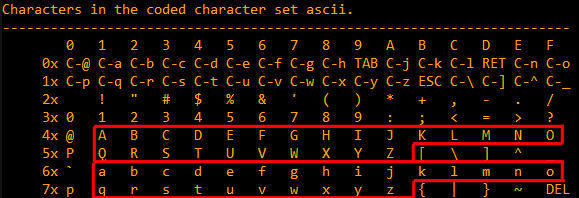
\includegraphics[width=0.7\textwidth]{ascii.png}
\caption{7-битная таблица \ac{ASCII} в Emacs}
\end{figure}

В десятичном виде этот бит это 32 \dots 32?
Но 32 это ASCII-код пробела!

Действительно, можно менять регистр просто применяя XOR к ASCII-коду, с 32 (больше об этом: \myref{toupper_bit}).

Возможно ли, что пустые лакуны в файле это не нулевые байты, а скорее содержащие пробелы?
Еще раз модифицируем наш XOR-ключ (я про-XOR-ю каждый байт ключа с 32):

\begin{lstlisting}[style=custommath]
(* "32" это скаляр, и "key" это вектор, но это OK *)

In[]:= key3 = BitXor[32, key]
Out[]= {112, 86, 34, 84, 81, 70, 86, 57, 67, 40, 51, 55, 84, 93, 75, \
57, 67, 77, 82, 70, 46, 89, 83, 63, 41, 85, 81, 79, 37, 36, 95, 60, \
90, 69, 40, 78, 46, 50, 92, 74, 48, 52, 72, 87, 40, 77, 58, 74, 41, \
65, 45, 67, 47, 87, 52, 73, 85, 66, 71, 86, 33, 94, 61, 65, 90, 49, \
47, 82, 78, 35, 37, 93, 93, 67, 94, 87, 70, 62, 90, 34, 85}

In[]:= DecryptBlock[blk_] := BitXor[key3, blk]
\end{lstlisting}

И снова дешифруем входной файл:

\begin{figure}[H]
\centering
\myincludegraphics{ff/XOR/mask_1/mc_decrypted.png}
\caption{Дешифрованный файл в Midnight Commander, последняя попытка}
\end{figure}

(Расшифрованный файл доступен здесь:
\url{https://github.com/dennis714/RE-for-beginners/blob/master/ff/XOR/mask_1/files/decrypted.dat.bz2}.)

Несомненно, это корректный исходный файл.
Да, и мы видим числа в начале каждого блока. Должно быть это и есть источник некорректного XOR-ключа.
Как выходит, самый встречающийся 81-байтный блок в файле это блок заполненный пробелами и содержащий символ \q{1} на месте
второго байта.
Действительно, как-то так получилось что многие блоки здесь перемежаются с этим блоком.
Может быть это что-то вроде выравнивания (padding) для коротких фраз/сообщений?
Другой часто встречающийся 81-байтный блок также заполнен пробелами, но с другой цифрой, следовательно,
они отличаются только вторым байтом.

Вот и всё! Теперь мы можем написать утилиту для зашифрования файла назад, и, может быть, модифицировать его перед этим

Файл для Mathematica можно скачать здесь:
\url{https://github.com/dennis714/RE-for-beginners/blob/master/ff/XOR/mask_1/files/XOR_mask_1.nb}.

Итог: XOR-шифрование не надежно вообще. Вероятно, разработчик игры хотел просто скрыть внутренности игры от игрока,
ничего более серьезного.
Все же, шифрование вроде этого крайне популярно вследствии его простоты, так что многие реверс инженеры обычно хорошо
с этим знакомы.

}
\EN{% TODO translate
\subsection{Simple encryption using XOR mask, case II}
\label{XOR_mask_2}

I've got another encrypted file, which is clearly encrypted by something simple, like XOR-ing:

\begin{figure}[H]
\centering
\myincludegraphics{ff/XOR/mask_2/cipher.png}
\caption{Encrypted file in Midnight Commander}
\end{figure}

The encrypted file can be downloaded \href{https://github.com/dennis714/RE-for-beginners/blob/master/ff/XOR/mask_2/files/cipher.txt}{here}.

\IT{ent} Linux utility reports about $\textasciitilde{}7.5$ bits per byte, and this is high level of entropy (\myref{entropy}),
close to compressed or properly encrypted file.
But still, we clearly see some pattern, there are some blocks with size of 17 bytes, hence, you see some kind of ladder,
shifting by 1 byte at each 16-byte line.

It's also known that the plain text is just English language text.

Now let's assume that this piece of text is encrypted by simple XOR-ing with 17-byte key.

I tried to find some repeating 17-byte blocks in Mathematica, like I did before in my previous example (\myref{XOR_mask_1}):

\begin{lstlisting}[caption=Mathematica,style=custommath]
In[]:=input = BinaryReadList["/home/dennis/tmp/cipher.txt"];

In[]:=blocks = Partition[input, 17];

In[]:=Sort[Tally[blocks], #1[[2]] > #2[[2]] &]

Out[]:={{{248,128,88,63,58,175,159,154,232,226,161,50,97,127,3,217,80},1},
{{226,207,67,60,42,226,219,150,246,163,166,56,97,101,18,144,82},1},
{{228,128,79,49,59,250,137,154,165,236,169,118,53,122,31,217,65},1},
{{252,217,1,39,39,238,143,223,241,235,170,91,75,119,2,152,82},1},
{{244,204,88,112,59,234,151,147,165,238,170,118,49,126,27,144,95},1},
{{241,196,78,112,54,224,142,223,242,236,186,58,37,50,17,144,95},1},
{{176,201,71,112,56,230,143,151,234,246,187,118,44,125,8,156,17},1},
...
{{255,206,82,112,56,231,158,145,165,235,170,118,54,115,9,217,68},1},
{{249,206,71,34,42,254,142,154,235,247,239,57,34,113,27,138,88},1},
{{157,170,84,32,32,225,219,139,237,236,188,51,97,124,21,141,17},1},
{{248,197,1,61,32,253,149,150,235,228,188,122,97,97,27,143,84},1},
{{252,217,1,38,42,253,130,223,233,226,187,51,97,123,20,217,69},1},
{{245,211,13,112,56,231,148,223,242,226,188,118,52,97,15,152,93},1},
{{221,210,15,112,28,231,158,141,233,236,172,61,97,90,21,149,92},1}}
\end{lstlisting}

No luck, each 17-byte block is unique within the file and occurred only once.
Perhaps, there are no 17-byte zero (or space) lacunas.
It is possible indeed: such long space indentation and padding may be absent in tightly typeset text.

The first idea is to try all possible 17-byte keys and find those, which will result in printable plain text after decryption.
Bruteforce is not an option, because there are $256^{17}$ possible keys ($\textasciitilde{}10^{40}$), that's too much.
But there are good news: who said we have to test 17-byte key as a whole, why can't we test each byte of key separately?
It is possible indeed.

Now the algorithm is:

\begin{itemize}
\item try all 256 bytes for 1st byte of key;
\item decrypt 1st byte of each 17-byte blocks in the file;
\item are all decrypted bytes we got are printable? keep tabs on it;
\item do so for all 17 bytes of key.
\end{itemize}

I've wrotten the following Python script to check this idea:

\begin{lstlisting}[caption=Python script,style=custompy]
each_Nth_byte=[""]*KEY_LEN

content=read_file(sys.argv[1])
# split input by 17-byte chunks:
all_chunks=chunks(content, KEY_LEN)
for c in all_chunks:
    for i in range(KEY_LEN):
        each_Nth_byte[i]=each_Nth_byte[i] + c[i]

# try each byte of key
for N in range(KEY_LEN):
    print "N=", N
    possible_keys=[]
    for i in range(256):
        tmp_key=chr(i)*len(each_Nth_byte[N])
        tmp=xor_strings(tmp_key,each_Nth_byte[N])
        # are all characters in tmp[] are printable?
        if is_string_printable(tmp)==False:
	    continue
	possible_keys.append(i)
    print possible_keys, "len=", len(possible_keys)
\end{lstlisting}

(Full version of the source code is \href{https://github.com/dennis714/RE-for-beginners/blob/master/ff/XOR/mask_2/files/decrypt2.py}{here}.)

Here is its output:

\begin{lstlisting}
N= 0
[144, 145, 151] len= 3
N= 1
[160, 161] len= 2
N= 2
[32, 33, 38] len= 3
N= 3
[80, 81, 87] len= 3
N= 4
[78, 79] len= 2
N= 5
[142, 143] len= 2
N= 6
[250, 251] len= 2
N= 7
[254, 255] len= 2
N= 8
[130, 132, 133] len= 3
N= 9
[130, 131] len= 2
N= 10
[206, 207] len= 2
N= 11
[81, 86, 87] len= 3
N= 12
[64, 65] len= 2
N= 13
[18, 19] len= 2
N= 14
[122, 123] len= 2
N= 15
[248, 249] len= 2
N= 16
[48, 49] len= 2
\end{lstlisting}

So there are 2 or 3 possible bytes for each byte of 17-byte key.
This is much better than 256 possible bytes for each byte, but still too much.
There are up to 1 million of possible keys:

\begin{lstlisting}[caption=Mathematica,style=custommath]
In[]:= 3*2*3*3*2*2*2*2*3*2*2*3*2*2*2*2*2
Out[]= 995328
\end{lstlisting}

It's possible to check all of them, but then we must check visually, if the decrypted text is looks like English language text.

Let's also take into consideration the fact that we deal with 1) natural language; 2) English language.
Natural languages has some prominent statistical features.
First of all, punctuation and word lengths.
What is average word length in English language?
Let's just count spaces in some well-known English language texts using Mathematica.

Here is \href{http://www.gutenberg.org/cache/epub/100/pg100.txt}{\q{The Complete Works of William Shakespeare}} text file from Gutenberg Library:

\begin{lstlisting}[caption=Mathematica,style=custommath]
In[]:= input = BinaryReadList["/home/dennis/tmp/pg100.txt"];

In[]:= Tally[input]
Out[]= {{239, 1}, {187, 1}, {191, 1}, {84, 39878}, {104, 
  218875}, {101, 406157}, {32, 1285884}, {80, 12038}, {114, 
  209907}, {111, 282560}, {106, 2788}, {99, 67194}, {116, 
  291243}, {71, 11261}, {117, 115225}, {110, 216805}, {98, 
  46768}, {103, 57328}, {69, 42703}, {66, 15450}, {107, 29345}, {102, 
  69103}, {67, 21526}, {109, 95890}, {112, 46849}, {108, 146532}, {87,
   16508}, {115, 215605}, {105, 199130}, {97, 245509}, {83, 
  34082}, {44, 83315}, {121, 85549}, {13, 124787}, {10, 124787}, {119,
   73155}, {100, 134216}, {118, 34077}, {46, 78216}, {89, 9128}, {45, 
  8150}, {76, 23919}, {42, 73}, {79, 33268}, {82, 29040}, {73, 
  55893}, {72, 18486}, {68, 15726}, {58, 1843}, {65, 44560}, {49, 
  982}, {50, 373}, {48, 325}, {91, 2076}, {35, 3}, {93, 2068}, {74, 
  2071}, {57, 966}, {52, 107}, {70, 11770}, {85, 14169}, {78, 
  27393}, {75, 6206}, {77, 15887}, {120, 4681}, {33, 8840}, {60, 
  468}, {86, 3587}, {51, 343}, {88, 608}, {40, 643}, {41, 644}, {62, 
  440}, {39, 31077}, {34, 488}, {59, 17199}, {126, 1}, {95, 71}, {113,
   2414}, {81, 1179}, {63, 10476}, {47, 48}, {55, 45}, {54, 73}, {64, 
  3}, {53, 94}, {56, 47}, {122, 1098}, {90, 532}, {124, 33}, {38, 
  21}, {96, 1}, {125, 2}, {37, 1}, {36, 2}}

In[]:= Length[input]/1285884 // N
Out[]= 4.34712
\end{lstlisting}

There are 1285884 spaces in the whole file, and the frequency of space occurrence is 1 space per
$\textasciitilde{}4.3$ characters.

Now here is \href{http://www.gutenberg.org/ebooks/11}{Alice's Adventures in Wonderland, by Lewis Carroll}
from the same library:

\begin{lstlisting}[caption=Mathematica,style=custommath]
In[]:= input = BinaryReadList["/home/dennis/tmp/pg11.txt"];

In[]:= Tally[input]
Out[]= {{239, 1}, {187, 1}, {191, 1}, {80, 172}, {114, 6398}, {111, 
  9243}, {106, 222}, {101, 15082}, {99, 2815}, {116, 11629}, {32, 
  27964}, {71, 193}, {117, 3867}, {110, 7869}, {98, 1621}, {103, 
  2750}, {39, 2885}, {115, 6980}, {65, 721}, {108, 5053}, {105, 
  7802}, {100, 5227}, {118, 911}, {87, 256}, {97, 9081}, {44, 
  2566}, {121, 2442}, {76, 158}, {119, 2696}, {67, 185}, {13, 
  3735}, {10, 3735}, {84, 571}, {104, 7580}, {66, 125}, {107, 
  1202}, {102, 2248}, {109, 2245}, {46, 1206}, {89, 142}, {112, 
  1796}, {45, 744}, {58, 255}, {68, 242}, {74, 13}, {50, 12}, {53, 
  13}, {48, 22}, {56, 10}, {91, 4}, {69, 313}, {35, 1}, {49, 68}, {93,
   4}, {82, 212}, {77, 222}, {57, 11}, {52, 10}, {42, 88}, {83, 
  288}, {79, 234}, {70, 134}, {72, 309}, {73, 831}, {85, 111}, {78, 
  182}, {75, 88}, {86, 52}, {51, 13}, {63, 202}, {40, 76}, {41, 
  76}, {59, 194}, {33, 451}, {113, 135}, {120, 170}, {90, 1}, {122, 
  79}, {34, 135}, {95, 4}, {81, 85}, {88, 6}, {47, 24}, {55, 6}, {54, 
  7}, {37, 1}, {64, 2}, {36, 2}}

In[]:= Length[input]/27964 // N
Out[]= 5.99049
\end{lstlisting}

The result is different probably because of different formatting of these texts (maybe indentation and/or padding).

OK, so let's assume the average frequency of space in English language is 1 space per 4..7 characters.

Now the good news again: we can measure frequency of spaces while decrypting our file gradually.
Now I count spaces in each \IT{slice} and throw away 1-byte keys which produce buffers with too small number of spaces
(or too large, but this is almost impossible given so short key):

\begin{lstlisting}[caption=Python script,style=custompy]
each_Nth_byte=[""]*KEY_LEN

content=read_file(sys.argv[1])
# split input by 17-byte chunks:
all_chunks=chunks(content, KEY_LEN)
for c in all_chunks:
    for i in range(KEY_LEN):
        each_Nth_byte[i]=each_Nth_byte[i] + c[i]

# try each byte of key
for N in range(KEY_LEN):
    print "N=", N
    possible_keys=[]
    for i in range(256):
        tmp_key=chr(i)*len(each_Nth_byte[N])
        tmp=xor_strings(tmp_key,each_Nth_byte[N])
        # are all characters in tmp[] are printable?
        if is_string_printable(tmp)==False:
	    continue
        # count spaces in decrypted buffer:
	spaces=tmp.count(' ')
	if spaces==0:
            continue
	spaces_ratio=len(tmp)/spaces
	if spaces_ratio<4:
	    continue
	if spaces_ratio>7:
	    continue
	possible_keys.append(i)
    print possible_keys, "len=", len(possible_keys)
\end{lstlisting}

(Full version of the source code is \href{https://github.com/dennis714/RE-for-beginners/blob/master/ff/XOR/mask_2/files/decrypt3.py}{here}.)

This reports just one single possible byte for each byte of key:

\begin{lstlisting}
N= 0
[144] len= 1
N= 1
[160] len= 1
N= 2
[33] len= 1
N= 3
[80] len= 1
N= 4
[79] len= 1
N= 5
[143] len= 1
N= 6
[251] len= 1
N= 7
[255] len= 1
N= 8
[133] len= 1
N= 9
[131] len= 1
N= 10
[207] len= 1
N= 11
[86] len= 1
N= 12
[65] len= 1
N= 13
[18] len= 1
N= 14
[122] len= 1
N= 15
[249] len= 1
N= 16
[49] len= 1
\end{lstlisting}

Let's check this key in Mathematica:

\begin{lstlisting}[caption=Mathematica,style=custommath]
In[]:= input = BinaryReadList["/home/dennis/tmp/cipher.txt"];

In[]:= blocks = Partition[input, 17];

In[]:= key = {144, 160, 33, 80, 79, 143, 251, 255, 133, 131, 207, 86, 65, 18, 122, 249, 49};

In[]:= EncryptBlock[blk_] := BitXor[key, blk]

In[]:= encrypted = Map[EncryptBlock[#] &, blocks];

In[]:= BinaryWrite["/home/dennis/tmp/plain2.txt", Flatten[encrypted]]

In[]:= Close["/home/dennis/tmp/plain2.txt"]
\end{lstlisting}

And the plain text is:

\begin{lstlisting}
Mr. Sherlock Holmes, who was usually very late in the mornings, save
upon those not infrequent occasions when he was up all night, was seated
at the breakfast table. I stood upon the hearth-rug and picked up the
stick which our visitor had left behind him the night before. It was a
fine, thick piece of wood, bulbous-headed, of the sort which is known as
a "Penang lawyer." Just under the head was a broad silver band nearly
an inch across. "To James Mortimer, M.R.C.S., from his friends of the
C.C.H.," was engraved upon it, with the date "1884." It was just such a
stick as the old-fashioned family practitioner used to carry--dignified,
solid, and reassuring.

"Well, Watson, what do you make of it?"

Holmes was sitting with his back to me, and I had given him no sign of
my occupation.

...
\end{lstlisting}

(Full version of the text is \href{https://github.com/dennis714/RE-for-beginners/blob/master/ff/XOR/mask_2/files/plain.txt}{here}.)

The text looks correct.
Yes, I made up this example and choose well-known text of Conan Doyle, but it's very close to what I had in my practice some time ago.

\subsubsection{Other ideas to consider}

If we would fail with space counting, there are other ideas to try:

\begin{itemize}

\item Take into consideration the fact that lowercase letters are much more frequent than uppercase ones.

\item Frequency analysis.

\item There is also a good technique to detect language of a text: trigrams.
Each language has some very frequent letter triplets, these may be \q{the} and \q{tha} for English.
Read more about it:
\href{http://odur.let.rug.nl/~vannoord/TextCat/textcat.pdf}{N-Gram-Based Text Categorization},
\url{http://code.activestate.com/recipes/326576/}.
Interestingly enough, trigrams detection can be used when you decrypt a ciphertext gradually,
like in this example (you just have to test 3 adjacent decrypted characters).

For non-Latin writing systems encoded in UTF-8, things may be easier.
For example, Russian text encoded in UTF-8 has each byte interleaved with 0xD0/0xD1 byte.
It is because Cyrillic characters are placed in 4th block of Unicode table.
Other writing systems has their own blocks.

\end{itemize}

}\RU{% TODO translate
\subsection{Простое шифрование используя XOR-маску, второй случай}
\label{XOR_mask_2}

Нашел еще один зашифрованный файл, который явно зашифрован чем-то простым вроде XOR-шифрования:

\begin{figure}[H]
\centering
\myincludegraphics{ff/XOR/mask_2/cipher.png}
\caption{Зашифрованный файл в Midnight Commander}
\end{figure}

Зашифрованный файл можно скачать \href{https://github.com/dennis714/RE-for-beginners/blob/master/ff/XOR/mask_2/files/cipher.txt}{здесь}.

Утилита \IT{ent} в Linux сообщает о $\textasciitilde{}7.5$ бит на байт, и это высокий уровень энтропии (\myref{entropy}),
что близко к сжатому или правильно зашифрованному файлу.
Но все-таки, мы ясно видим некоторый шаблон, здесь есть блоки длиной в 17 байт, и вы можете увидеть что-то вроде лестницы,
сдвигающеся на 1 байт на каждой 16-байтной линии.

Также известно, что исходный текст это текст на английском языке.

Предположим что этот фрагмент текста зашифрован простым XOR-шифрованием с 17-байтным ключом.

Я попробовал поискать повторяющиеся 17-байтные блоки при помощи Mathematica, как я делал это в моем предыдущем примере
(\myref{XOR_mask_1}):

\begin{lstlisting}[caption=Mathematica,style=custommath]
In[]:=input = BinaryReadList["/home/dennis/tmp/cipher.txt"];

In[]:=blocks = Partition[input, 17];

In[]:=Sort[Tally[blocks], #1[[2]] > #2[[2]] &]

Out[]:={{{248,128,88,63,58,175,159,154,232,226,161,50,97,127,3,217,80},1},
{{226,207,67,60,42,226,219,150,246,163,166,56,97,101,18,144,82},1},
{{228,128,79,49,59,250,137,154,165,236,169,118,53,122,31,217,65},1},
{{252,217,1,39,39,238,143,223,241,235,170,91,75,119,2,152,82},1},
{{244,204,88,112,59,234,151,147,165,238,170,118,49,126,27,144,95},1},
{{241,196,78,112,54,224,142,223,242,236,186,58,37,50,17,144,95},1},
{{176,201,71,112,56,230,143,151,234,246,187,118,44,125,8,156,17},1},
...
{{255,206,82,112,56,231,158,145,165,235,170,118,54,115,9,217,68},1},
{{249,206,71,34,42,254,142,154,235,247,239,57,34,113,27,138,88},1},
{{157,170,84,32,32,225,219,139,237,236,188,51,97,124,21,141,17},1},
{{248,197,1,61,32,253,149,150,235,228,188,122,97,97,27,143,84},1},
{{252,217,1,38,42,253,130,223,233,226,187,51,97,123,20,217,69},1},
{{245,211,13,112,56,231,148,223,242,226,188,118,52,97,15,152,93},1},
{{221,210,15,112,28,231,158,141,233,236,172,61,97,90,21,149,92},1}}
\end{lstlisting}

Ничего не выходит, каждый 17-байтный блок уникален внутри файла и встречается только один раз.
Возможно, здесь нет 17-байтных нулевых лакун (или лакун содержащих пробелы).
Это действительно возможно: подобное выравнивание пробелами может и отсутствовать в плотно сверстаном тексте.

Первая идея это попробовать все возможные 17-байтные ключи и найти тот, который после дешифровки приведет к читаемому тексту.
Полный перебор брутфорсом это не вариант, потому что здесь $256^{17}$ возможных ключей ($\textasciitilde{}10^{40}$),
это слишком.
Но есть и хорошие новости: кто сказал что нужно тестировать 17-байтный ключ как что-то целое, почему мы не можем тестировать
каждый байт ключа отдельно?
Это действительно возможно.

И алгоритм такой:

\begin{itemize}
\item попробовать все 256 байт для первого байта ключа;
\item дешифровать первый байт каждого 17-байтного блока в файле;
\item все ли полученные дешифрованные байты печатаемы? вести учет;
\item делать это для всех 17 байт ключа.
\end{itemize}

Я написал такой скрипт на Питоне для проверки этой идеи:

\begin{lstlisting}[caption=Python script,style=custompy]
each_Nth_byte=[""]*KEY_LEN

content=read_file(sys.argv[1])
# split input by 17-byte chunks:
all_chunks=chunks(content, KEY_LEN)
for c in all_chunks:
    for i in range(KEY_LEN):
        each_Nth_byte[i]=each_Nth_byte[i] + c[i]

# try each byte of key
for N in range(KEY_LEN):
    print "N=", N
    possible_keys=[]
    for i in range(256):
        tmp_key=chr(i)*len(each_Nth_byte[N])
        tmp=xor_strings(tmp_key,each_Nth_byte[N])
        # are all characters in tmp[] are printable?
        if is_string_printable(tmp)==False:
	    continue
	possible_keys.append(i)
    print possible_keys, "len=", len(possible_keys)
\end{lstlisting}

(Полная версия исходного кода \href{https://github.com/dennis714/RE-for-beginners/blob/master/ff/XOR/mask_2/files/decrypt2.py}{здесь}.)

И вот вывод:

\begin{lstlisting}
N= 0
[144, 145, 151] len= 3
N= 1
[160, 161] len= 2
N= 2
[32, 33, 38] len= 3
N= 3
[80, 81, 87] len= 3
N= 4
[78, 79] len= 2
N= 5
[142, 143] len= 2
N= 6
[250, 251] len= 2
N= 7
[254, 255] len= 2
N= 8
[130, 132, 133] len= 3
N= 9
[130, 131] len= 2
N= 10
[206, 207] len= 2
N= 11
[81, 86, 87] len= 3
N= 12
[64, 65] len= 2
N= 13
[18, 19] len= 2
N= 14
[122, 123] len= 2
N= 15
[248, 249] len= 2
N= 16
[48, 49] len= 2
\end{lstlisting}

Так что есть 2 или 3 возможных байта для каждого байта 17-байтного ключа.
Это намного лучше чем 256 возможных байт для каждого ключа, но все равно слишком.
Тут вплоть до одного миллиона возможных ключей:

\begin{lstlisting}[caption=Mathematica,style=custommath]
In[]:= 3*2*3*3*2*2*2*2*3*2*2*3*2*2*2*2*2
Out[]= 995328
\end{lstlisting}

Можно проверить их все, но затем нам придется проверять визуально, похож ли дешифрованный текст на текст на английском языке.

Также будет учитывать те факты, что мы имеем дело с 1) человеческим языком; 2) английским языком.
Человеческие языки имеют выдающиеся статистические особенности.
Прежде всего, пунктуация и длины слов.
Какая средняя длина слова в английском языке?
Просто будем считать пробелы в некоторых хорошо известных текстах на английском используя Mathematica.

Вот текст is \href{http://www.gutenberg.org/cache/epub/100/pg100.txt}{\q{The Complete Works of William Shakespeare}}
из библиотеки Гутенберга:

\begin{lstlisting}[caption=Mathematica,style=custommath]
In[]:= input = BinaryReadList["/home/dennis/tmp/pg100.txt"];

In[]:= Tally[input]
Out[]= {{239, 1}, {187, 1}, {191, 1}, {84, 39878}, {104, 
  218875}, {101, 406157}, {32, 1285884}, {80, 12038}, {114, 
  209907}, {111, 282560}, {106, 2788}, {99, 67194}, {116, 
  291243}, {71, 11261}, {117, 115225}, {110, 216805}, {98, 
  46768}, {103, 57328}, {69, 42703}, {66, 15450}, {107, 29345}, {102, 
  69103}, {67, 21526}, {109, 95890}, {112, 46849}, {108, 146532}, {87,
   16508}, {115, 215605}, {105, 199130}, {97, 245509}, {83, 
  34082}, {44, 83315}, {121, 85549}, {13, 124787}, {10, 124787}, {119,
   73155}, {100, 134216}, {118, 34077}, {46, 78216}, {89, 9128}, {45, 
  8150}, {76, 23919}, {42, 73}, {79, 33268}, {82, 29040}, {73, 
  55893}, {72, 18486}, {68, 15726}, {58, 1843}, {65, 44560}, {49, 
  982}, {50, 373}, {48, 325}, {91, 2076}, {35, 3}, {93, 2068}, {74, 
  2071}, {57, 966}, {52, 107}, {70, 11770}, {85, 14169}, {78, 
  27393}, {75, 6206}, {77, 15887}, {120, 4681}, {33, 8840}, {60, 
  468}, {86, 3587}, {51, 343}, {88, 608}, {40, 643}, {41, 644}, {62, 
  440}, {39, 31077}, {34, 488}, {59, 17199}, {126, 1}, {95, 71}, {113,
   2414}, {81, 1179}, {63, 10476}, {47, 48}, {55, 45}, {54, 73}, {64, 
  3}, {53, 94}, {56, 47}, {122, 1098}, {90, 532}, {124, 33}, {38, 
  21}, {96, 1}, {125, 2}, {37, 1}, {36, 2}}

In[]:= Length[input]/1285884 // N
Out[]= 4.34712
\end{lstlisting}

Тут 1285884 пробела во всем файле, и распространение пробелов это один пробел на $\textasciitilde{}4.3$ символов.

Теперь вот \href{http://www.gutenberg.org/ebooks/11}{Alice's Adventures in Wonderland, by Lewis Carroll} из той же библиотеки:

\begin{lstlisting}[caption=Mathematica,style=custommath]
In[]:= input = BinaryReadList["/home/dennis/tmp/pg11.txt"];

In[]:= Tally[input]
Out[]= {{239, 1}, {187, 1}, {191, 1}, {80, 172}, {114, 6398}, {111, 
  9243}, {106, 222}, {101, 15082}, {99, 2815}, {116, 11629}, {32, 
  27964}, {71, 193}, {117, 3867}, {110, 7869}, {98, 1621}, {103, 
  2750}, {39, 2885}, {115, 6980}, {65, 721}, {108, 5053}, {105, 
  7802}, {100, 5227}, {118, 911}, {87, 256}, {97, 9081}, {44, 
  2566}, {121, 2442}, {76, 158}, {119, 2696}, {67, 185}, {13, 
  3735}, {10, 3735}, {84, 571}, {104, 7580}, {66, 125}, {107, 
  1202}, {102, 2248}, {109, 2245}, {46, 1206}, {89, 142}, {112, 
  1796}, {45, 744}, {58, 255}, {68, 242}, {74, 13}, {50, 12}, {53, 
  13}, {48, 22}, {56, 10}, {91, 4}, {69, 313}, {35, 1}, {49, 68}, {93,
   4}, {82, 212}, {77, 222}, {57, 11}, {52, 10}, {42, 88}, {83, 
  288}, {79, 234}, {70, 134}, {72, 309}, {73, 831}, {85, 111}, {78, 
  182}, {75, 88}, {86, 52}, {51, 13}, {63, 202}, {40, 76}, {41, 
  76}, {59, 194}, {33, 451}, {113, 135}, {120, 170}, {90, 1}, {122, 
  79}, {34, 135}, {95, 4}, {81, 85}, {88, 6}, {47, 24}, {55, 6}, {54, 
  7}, {37, 1}, {64, 2}, {36, 2}}

In[]:= Length[input]/27964 // N
Out[]= 5.99049
\end{lstlisting}

Результат другой, вероятно потому что используется разное форматирование этих текстов (может быть из-за выравнивания
и отступов).

ОК, будем считать что средняя частота появления пробела в английском тексте это 1 пробел на 4..7 символов.

И снова хорошие новости: мы можем измерять частоту пробелов во время постепенного дешифрования файла.
Теперь я считаю пробелы в каждом \IT{ломтике} и выкидываю 1-байтные ключи, которые приводят к результатам со слишком
малым количеством пробелов
(или слишком большим, но это почти невозможно учитывая такой короткий ключ):

\begin{lstlisting}[caption=Python script,style=custompy]
each_Nth_byte=[""]*KEY_LEN

content=read_file(sys.argv[1])
# split input by 17-byte chunks:
all_chunks=chunks(content, KEY_LEN)
for c in all_chunks:
    for i in range(KEY_LEN):
        each_Nth_byte[i]=each_Nth_byte[i] + c[i]

# try each byte of key
for N in range(KEY_LEN):
    print "N=", N
    possible_keys=[]
    for i in range(256):
        tmp_key=chr(i)*len(each_Nth_byte[N])
        tmp=xor_strings(tmp_key,each_Nth_byte[N])
        # are all characters in tmp[] are printable?
        if is_string_printable(tmp)==False:
	    continue
        # count spaces in decrypted buffer:
	spaces=tmp.count(' ')
	if spaces==0:
            continue
	spaces_ratio=len(tmp)/spaces
	if spaces_ratio<4:
	    continue
	if spaces_ratio>7:
	    continue
	possible_keys.append(i)
    print possible_keys, "len=", len(possible_keys)
\end{lstlisting}

(Полная версия исходного кода \href{https://github.com/dennis714/RE-for-beginners/blob/master/ff/XOR/mask_2/files/decrypt3.py}{здесь}.)

Это выдает всего один возможный байт для каждого байта ключа:

\begin{lstlisting}
N= 0
[144] len= 1
N= 1
[160] len= 1
N= 2
[33] len= 1
N= 3
[80] len= 1
N= 4
[79] len= 1
N= 5
[143] len= 1
N= 6
[251] len= 1
N= 7
[255] len= 1
N= 8
[133] len= 1
N= 9
[131] len= 1
N= 10
[207] len= 1
N= 11
[86] len= 1
N= 12
[65] len= 1
N= 13
[18] len= 1
N= 14
[122] len= 1
N= 15
[249] len= 1
N= 16
[49] len= 1
\end{lstlisting}

Проверим этот ключ в Mathematica:

\begin{lstlisting}[caption=Mathematica,style=custommath]
In[]:= input = BinaryReadList["/home/dennis/tmp/cipher.txt"];

In[]:= blocks = Partition[input, 17];

In[]:= key = {144, 160, 33, 80, 79, 143, 251, 255, 133, 131, 207, 86, 65, 18, 122, 249, 49};

In[]:= EncryptBlock[blk_] := BitXor[key, blk]

In[]:= encrypted = Map[EncryptBlock[#] &, blocks];

In[]:= BinaryWrite["/home/dennis/tmp/plain2.txt", Flatten[encrypted]]

In[]:= Close["/home/dennis/tmp/plain2.txt"]
\end{lstlisting}

И дешифрованный текст:

\begin{lstlisting}
Mr. Sherlock Holmes, who was usually very late in the mornings, save
upon those not infrequent occasions when he was up all night, was seated
at the breakfast table. I stood upon the hearth-rug and picked up the
stick which our visitor had left behind him the night before. It was a
fine, thick piece of wood, bulbous-headed, of the sort which is known as
a "Penang lawyer." Just under the head was a broad silver band nearly
an inch across. "To James Mortimer, M.R.C.S., from his friends of the
C.C.H.," was engraved upon it, with the date "1884." It was just such a
stick as the old-fashioned family practitioner used to carry--dignified,
solid, and reassuring.

"Well, Watson, what do you make of it?"

Holmes was sitting with his back to me, and I had given him no sign of
my occupation.

...
\end{lstlisting}

(Полная версия текста \href{https://github.com/dennis714/RE-for-beginners/blob/master/ff/XOR/mask_2/files/plain.txt}{здесь}.)

Текст выглядит правильным.
Да, я придумал этот пример и выбрал хорошо известный текст Конан Дойля, но это очень близко к тому,
что у меня недавно было на практике.

\subsubsection{Другие идеи}

Если бы не получилось с подсчетом пробелов, вот еще идеи, которые можно было бы попробовать:

\begin{itemize}

\item Учитывать тот факт что буквы в нижнем регистре встречаются намного чаще, чем в верхнем.

\item Частотный анализ.

\item Есть очень хорошая техника для определения языка текста: триграммы.
Каждый язык имеет часто встречающиеся тройки буквы, для английского это могут быть \q{the} и \q{tha}.
Больше об этом:
\href{http://odur.let.rug.nl/~vannoord/TextCat/textcat.pdf}{N-Gram-Based Text Categorization},
\url{http://code.activestate.com/recipes/326576/}.
Интересно знать, что выявление триграмм может быть использовано при постепенном дешифровании текста, как в этом примере
(нужно просто проверять 3 рядом стоящих дешифрованных символа).

Для систем письменности отличных от латинского алфавита, закодированных в UTF-8, все может быть еще проще.
Например, в тексте на русском, закодированном в UTF-8, каждый байт перемежается с байтом 0xD0 или 0xD1.
Это потому что символы кириллицы расположен в 4-м блоке в таблице Уникода.
Другие системы письменности имеют свои блоки.

\end{itemize}

}


\EN{% TODO png blur? too wide listings
% TODO separate section for Mathematica example
\section[Analyzing using information entropy]{Analyzing unknown binary files using information entropy}
\label{entropy}
\myindex{Entropy}

For the sake of simplification, I would say, information entropy is a measure, how tightly some piece of data can be compressed.
For example, it is usually not possible to compress already compressed archive file, so it has high entropy.
On the other hand, one megabyte of zero bytes can be compressed to a tiny output file.
Indeed, in plain English language, one million of zeros can be described just as ``resulting file is one million zero bytes''.
Compressed files are usually a list of instructions to decompressor, like this: ``put 1000 zeros, then 0x23 byte, then 0x45 byte, then put a block of size 10 bytes which we've seen 500 bytes back, etc.''

Texts written in natural languages are also can be compressed tightly, 
because natural languages has a lot of redundancy
(otherwise, a tiny typo will always lead to misunderstanding, 
like any toggled bit in compressed archive make decompression nearly impossible), 
some words are used very often, etc.
It's possible to drop some words and text will be still readable.

Code for CPUs is also can be compressed, because some ISA instructions are used much more often than others.
\myindex{x86!\Instructions!MOV}
\myindex{x86!\Instructions!PUSH}
\myindex{x86!\Instructions!CALL}
In x86, most used instructions are MOV/PUSH/CALL---indeed, most of the time, computer CPU is just shuffling data and switching between
levels of abstractions.
If to consider data shuffling as moving data between levels of abstractions, this is also part of switching.

Data compressors and encryptors tend to produce very high entropy results.
Good pseudorandom number generators also produce data which cannot be compressed 
(it is possible to measure their quality by this sign).

So, in other words, entropy is a measure which can help to probe unknown data block.

\subsection{Analyzing entropy in Mathematica}

(This part has been first appeared in my blog at 13-May-2015.
Some discussion: \url{https://news.ycombinator.com/item?id=9545276}.)

It is possible to slice some file by blocks, probe each and draw a graph a graph.
I did this in Wolfram Mathematica for demonstration and here is a source code (Mathematica 10):

\begin{lstlisting}
(* loading the file *)
input=BinaryReadList["file.bin"];

(* setting block sizes *)
BlockSize=4096;BlockSizeToShow=256;

(* slice blocks by 4k *)
blocks=Partition[input,BlockSize];

(* how many blocks we've got? *)
Length[blocks]

(* calculate entropy for each block. 2 in Entropy[] (base) is set with the intention so Entropy[] 
function will produce the same results as Linux ent utility does *)
entropies=Map[N[Entropy[2,#]]&,blocks];

(* helper functions *)
fBlockToShow[input_,offset_]:=Take[input,{1+offset,1+offset+BlockSizeToShow}]
fToASCII[val_]:=FromCharacterCode[val,"PrintableASCII"]
fToHex[val_]:=IntegerString[val,16]
fPutASCIIWindow[data_]:=Framed[Grid[Partition[Map[fToASCII,data],16]]]
fPutHexWindow[data_]:=Framed[Grid[Partition[Map[fToHex,data],16],Alignment->Right]]

(* that will be the main knob here *)
{Slider[Dynamic[offset],{0,Length[input]-BlockSize,BlockSize}],Dynamic[BaseForm[offset,16]]}

(* main UI part *)
Dynamic[{ListLinePlot[entropies,GridLines->{{-1,offset/BlockSize,1}},Filling->Axis,AxesLabel->{"offset","entropy"}],
CurrentBlock=fBlockToShow[input,offset];
fPutHexWindow[CurrentBlock],
fPutASCIIWindow[CurrentBlock]}]
\end{lstlisting}

\subsubsection{GeoIP ISP database}

\myindex{GeoIP}
Let's start with the \href{https://www.maxmind.com/en/geoip-demo}{GeoIP} file (which assigns ISP to the block of IP addresses).
This binary file (\IT{GeoIPISP.dat}) has some tables (which are IP address ranges perhaps) plus some text blob at the end of the file
(containing ISP names).

When I load it to Mathematica, I see this:

\begin{figure}[H]
\centering
\myincludegraphics{ff/entropy/geoipisp1.png}
\end{figure}

There are two parts in graph: first is somewhat chaotic, second is more steady.

0 in horizontal axis in graph means lowest entropy (the data which can be compressed very tightly, \IT{ordered} in other words) 
and 8 is highest (cannot be compressed at all, \IT{chaotic} or \IT{random} in other words).
Why 0 and 8? 0 means 0 bits per byte (byte slot is not filled at all) 
and 8 means 8 bits per byte, i.e., the whole byte slot is filled with the information tightly.

So I put slider to point in the middle of the first block, and I clearly see some array of 32-bit integers.
Now I put slider in the middle of the second block and I see English text:

\begin{figure}[H]
\centering
\myincludegraphics{ff/entropy/geoipisp2.png}
\end{figure}

Indeed, this are names of ISPs.
So, entropy of English text is 4.5-5.5 bits per byte? Yes, something like this.
Wolfram Mathematica has some well-known English literature corpus embedded, and we can see entropy of Shakespeare's sonnets:

\begin{lstlisting}
In[]:= Entropy[2,ExampleData[{"Text","ShakespearesSonnets"}]]//N
Out[]= 4.42366
\end{lstlisting}

4.4 is close to what we've got (4.7-5.3). 
Of course, classic English literature texts are somewhat different from ISP names and other English texts we can find in binary files 
(debugging/logging/error messages), but this value is close.

\subsubsection{TP-Link WR941 firmware}

Now more complex example. I've got firmware for TP-Link WR941 router:

\begin{figure}[H]
\centering
\includegraphics[width=0.6\textwidth]{ff/entropy/tplink.png}
\end{figure}

Wee see here 3 blocks with empty lacunas.
The first block (started at address 0) is small, second (address somewhere at 0x22000) is bigger and third (address 0x123000) is biggest.
I can't be sure about exact entropy of the first block, but 2nd and 3rd has very high entropy, meaning that these blocks are either
compressed and/or encrypted.

\myindex{Binwalk}
I tried \href{http://binwalk.org/}{binwalk} for this firmware file:

\begin{lstlisting}
DECIMAL       HEXADECIMAL     DESCRIPTION
--------------------------------------------------------------------------------
0             0x0             TP-Link firmware header, firmware version: 0.-15221.3, image version: "", product ID: 0x0, product version: 155254789, kernel load address: 0x0, kernel entry point: 0x-7FFFE000, kernel offset: 4063744, kernel length: 512, rootfs offset: 837431, rootfs length: 1048576, bootloader offset: 2883584, bootloader length: 0
14832         0x39F0          U-Boot version string, "U-Boot 1.1.4 (Jun 27 2014 - 14:56:49)"
14880         0x3A20          CRC32 polynomial table, big endian
16176         0x3F30          uImage header, header size: 64 bytes, header CRC: 0x3AC66E95, created: 2014-06-27 06:56:50, image size: 34587 bytes, Data Address: 0x80010000, Entry Point: 0x80010000, data CRC: 0xDF2DBA0B, OS: Linux, CPU: MIPS, image type: Firmware Image, compression type: lzma, image name: "u-boot image"
16240         0x3F70          LZMA compressed data, properties: 0x5D, dictionary size: 33554432 bytes, uncompressed size: 90000 bytes
131584        0x20200         TP-Link firmware header, firmware version: 0.0.3, image version: "", product ID: 0x0, product version: 155254789, kernel load address: 0x0, kernel entry point: 0x-7FFFE000, kernel offset: 3932160, kernel length: 512, rootfs offset: 837431, rootfs length: 1048576, bootloader offset: 2883584, bootloader length: 0
132096        0x20400         LZMA compressed data, properties: 0x5D, dictionary size: 33554432 bytes, uncompressed size: 2388212 bytes
1180160       0x120200        Squashfs filesystem, little endian, version 4.0, compression:lzma, size: 2548511 bytes, 536 inodes, blocksize: 131072 bytes, created: 2014-06-27 07:06:52
\end{lstlisting}

\myindex{LZMA}
Indeed: there are some stuff at the beginning, but two large LZMA compressed blocks are started at 0x20400 and 0x120200.
These are roughly addresses we have seen in Mathematica.
Oh, and by the way, binwalk can show entropy information as well (-E option):

\begin{lstlisting}
DECIMAL       HEXADECIMAL     ENTROPY
--------------------------------------------------------------------------------
0             0x0             Falling entropy edge (0.419187)
16384         0x4000          Rising entropy edge (0.988639)
51200         0xC800          Falling entropy edge (0.000000)
133120        0x20800         Rising entropy edge (0.987596)
968704        0xEC800         Falling entropy edge (0.508720)
1181696       0x120800        Rising entropy edge (0.989615)
3727360       0x38E000        Falling entropy edge (0.732390)
\end{lstlisting}

Rising edges are corresponding to rising edges of block on our graph.
Falling edges are the points where empty lacunas are started.

I wasn't able to force binwalk to generate PNG graphs (due to absence of some Python library), but here is an example how binwalk
can do them: \url{http://binwalk.org/wp-content/uploads/2013/12/lg_dtv.png}.
% FIXME inline picture

What can we say about lacunas? By looking in hex editor, we see that these are just filled with 0xFF bytes.
Why developers put them? Perhaps, because they weren't able to calculate precise compressed blocks sizes, so they allocated space
for them with some reserve.

\subsubsection{Notepad}

\myindex{Notepad}

Another example is notepad.exe I've picked in Windows 8.1:

\begin{figure}[H]
\centering
\myincludegraphics{ff/entropy/notepad1.png}
\end{figure}

There is cavity at ~0x19000 (absolute file offset).
I opened the executable file in hex editor and found imports table there (which has lower entropy than x86-64 code
in the first half of graph).

There are also high entropy block started at ~0x20000:

\begin{figure}[H]
\centering
\myincludegraphics{ff/entropy/notepad2.png}
\end{figure}

\myindex{PNG}
In hex editor I can see PNG file here, embedded in the PE file resource section (it is a large image of notepad icon).
PNG files are compressed, indeed.

\subsubsection{Unnamed dashcam}

Now the most complex example in this article is the firmware of some unnamed dashcam I've received from friend:

\begin{figure}[H]
\centering
\myincludegraphics{ff/entropy/dashcam_text.png}
\end{figure}

The cavity at the very beginning is a English text: debugging messages.
\myindex{MIPS}
I checked various ISAs and I found that 
the first third of the whole file (with the text segment inside) is in fact MIPS (little-endian) code!

For instance, this is very distinctive MIPS function epilogue:

\begin{lstlisting}
ROM:000013B0                 move    $sp, $fp
ROM:000013B4                 lw      $ra, 0x1C($sp)
ROM:000013B8                 lw      $fp, 0x18($sp)
ROM:000013BC                 lw      $s1, 0x14($sp)
ROM:000013C0                 lw      $s0, 0x10($sp)
ROM:000013C4                 jr      $ra
ROM:000013C8                 addiu   $sp, 0x20
\end{lstlisting}

From our graph we can see that MIPS code has entropy of 5-6 bits per byte.
Indeed, I once measured various ISAs entropy and I've got these values:

\begin{itemize}
\item x86: .text section of ntoskrnl.exe file from Windows 2003: 6.6
\item x64: .text section of ntoskrnl.exe file from Windows 7 x64: 6.5
\item ARM (thumb mode), Angry Birds Classic: 7.05
\item ARM (ARM mode) Linux Kernel 3.8.0: 6.03
\item MIPS (little endian), .text section of user32.dll from Windows NT 4: 6.09
\end{itemize}

So the entropy of executable code is higher than of English text, but still can be compressed.

Now the second third is started at 0xF5000. I don't know what this is. I tried different ISAs but without success.
The entropy of the block is looks even steadier than for executable one.
Maybe some kind of data?

\myindex{JPEG}
There is also a spike at ~0x213000. I checked it in hex editor and I found JPEG file there 
(which, of course, compressed)!
I also don't know what is at the end.
Let's try Binwalk for this file:

\begin{lstlisting}
dennis@ubuntu:~/P/entropy$ binwalk FW96650A.bin 

DECIMAL       HEXADECIMAL     DESCRIPTION
--------------------------------------------------------------------------------
167698        0x28F12         Unix path: /15/20/24/25/30/60/120/240fps can be served..
280286        0x446DE         Copyright string: "Copyright (c) 2012 Novatek Microelectronic Corp."
2169199       0x21196F        JPEG image data, JFIF standard 1.01
2300847       0x231BAF        MySQL MISAM compressed data file Version 3

dennis@ubuntu:~/P/entropy$ binwalk -E FW96650A.bin 

WARNING: pyqtgraph not found, visual entropy graphing will be disabled

DECIMAL       HEXADECIMAL     ENTROPY
--------------------------------------------------------------------------------
0             0x0             Falling entropy edge (0.579792)
2170880       0x212000        Rising entropy edge (0.967373)
2267136       0x229800        Falling entropy edge (0.802974)
2426880       0x250800        Falling entropy edge (0.846639)
2490368       0x260000        Falling entropy edge (0.849804)
2560000       0x271000        Rising entropy edge (0.974340)
2574336       0x274800        Rising entropy edge (0.970958)
2588672       0x278000        Falling entropy edge (0.763507)
2592768       0x279000        Rising entropy edge (0.951883)
2596864       0x27A000        Falling entropy edge (0.712814)
2600960       0x27B000        Rising entropy edge (0.968167)
2607104       0x27C800        Rising entropy edge (0.958582)
2609152       0x27D000        Falling entropy edge (0.760989)
2654208       0x288000        Rising entropy edge (0.954127)
2670592       0x28C000        Rising entropy edge (0.967883)
2676736       0x28D800        Rising entropy edge (0.975779)
2684928       0x28F800        Falling entropy edge (0.744369)
\end{lstlisting}

Yes, it found JPEG file and even MySQL data!
But I'm not sure if it's true---I didn't check it yet.

\myindex{clusterization}
It's also interesting to try clusterization in Mathematica:

\begin{figure}[H]
\centering
\myincludegraphics{ff/entropy/dashcam_clusters.png}
\end{figure}

Here is an example of how Mathematica grouped various entropy values into distinctive groups.
Indeed, there is something credible. Blue dots in range of 5.0-5.5 are supposedly related to English text.
Yellow dots in 5.5-6 are MIPS code. A lot of green dots in 6.0-6.5 is the unknown second third.
Orange dots close to 8.0 are related to compressed JPEG file.
Other orange dots are supposedly related to the end of the firmware (unknown to us data).

\subsubsection{Links}

Binary files used while writing: \url{http://yurichev.com/blog/entropy/files/}.
Wolfram Mathematica notebook file: \url{http://yurichev.com/blog/entropy/files/binary_file_entropy.nb}
(all cells must be evaluated to start things working).



\subsection{Conclusion}

Information entropy can be used as a quick-n-dirty method for inspecting unknown binary files.
In particular, it is a very quick way to find compressed/encrypted pieces of data.
Someone say it's possible to find RSA (and other asymmetric cryptographic algorithms) public/private keys 
in executable code (which has high entropy as well), but I didn't try this myself.

\subsection{Tools}

Handy Linux \IT{ent} utility to measure entropy of a file\footnote{\url{http://www.fourmilab.ch/random/}}.

There is a great online entropy visualizer made by Aldo Cortesi, 
which I tried to mimic using Mathematica: \url{http://binvis.io}.
His articles about entropy visualization are worth reading:
\url{http://corte.si/posts/visualisation/entropy/index.html},
\url{http://corte.si/posts/visualisation/malware/index.html},
\url{http://corte.si/posts/visualisation/binvis/index.html}.

\myindex{radare2}
radare2 framework has \IT{\#entropy} command for this.

A tool for IDA: IDAtropy\footnote{\url{https://github.com/danigargu/IDAtropy}}.

\subsection{A word about primitive encryption like XORing}

It's interesting that simple XOR encryption doesn't affect entropy of data.
I've shown this in \IT{Norton Guide} example in the book (\myref{norton_guide}).

Generalizing: encryption by substitution cipher also doesn't affect entropy of data (and XOR can be viewed as substitution cipher).
The reason of that is because entropy calculation algorithm view data on byte-level.
On the other hand, the data encrypted by 2 or 4-byte XOR pattern will result in another entropy.

Nevertheless, low entropy is usually a good sign of weak amateur cryptography
(which is also used in license keys, license files, etc.).

\subsection{More about entropy of executable code}

It is quickly noticeable that probably a biggest source of high-entropy in executable code are relative offsets encoded in opcodes.
For example, these two consequent instructions will produce different relative offsets in their opcodes, 
while they are in fact pointing to the same function:

\begin{lstlisting}[style=customasm]
function proc
...
function endp

...

CALL function
...
CALL function
\end{lstlisting}

Ideal executable code compressor would encode information like this:
\IT{there is a CALL to a ``function'' at address X and the same CALL at address Y} without necessity to encode
address of the \IT{function} twice.

\myindex{UPX}
To deal with this, executable compressors are sometimes able to reduce entropy here.
One example is UPX: \url{http://sourceforge.net/p/upx/code/ci/default/tree/doc/filter.txt}.

\subsection{Random number generators}

\myindex{GnuPG}
When I run GnuPG to generate new secret key, it asking for some entropy...

\begin{lstlisting}
We need to generate a lot of random bytes. It is a good idea to perform
some other action (type on the keyboard, move the mouse, utilize the
disks) during the prime generation; this gives the random number
generator a better chance to gain enough entropy.

Not enough random bytes available.  Please do some other work to give
the OS a chance to collect more entropy! (Need 169 more bytes)
\end{lstlisting}

This means that good a PRNG produces long high-entropy results, and this is what the secret asymetrical cryptographical key needs.
But \ac{CPRNG} is tricky (because computer is highly deterministic device itself),
so the GnuPG asking for some additional randomness from the user.

Here is a case where I made attempt to calculate entropy of some unknown blocks: \myref{encrypted_DB1}.

\subsection{Entropy of various files}

Entropy of random bytes is close to 8:

\begin{lstlisting}[basicstyle=\ttfamily, mathescape]
$\$$ dd bs=1M count=1 if=/dev/urandom | ent
Entropy = 7.999803 bits per byte.
\end{lstlisting}

This means, almost all available space inside of byte is filled with information.

256 bytes in range of 0..255 gives exact value of 8:

\begin{lstlisting}[basicstyle=\ttfamily, mathescape,style=custompy]
#!/usr/bin/env python
import sys

for i in range(256):
    sys.stdout.write(chr(i))
\end{lstlisting}

\begin{lstlisting}[basicstyle=\ttfamily, mathescape]
python 1.py | ent
Entropy = 8.000000 bits per byte.
\end{lstlisting}

Order of bytes doesn't matter.
This means, all available space inside of byte is filled.

Entropy of all zero bytes is 0:

\begin{lstlisting}[basicstyle=\ttfamily, mathescape]
$\$$ dd bs=1M count=1 if=/dev/zero | ent
Entropy = 0.000000 bits per byte.
\end{lstlisting}

Entropy of a string costisting of a single (any) byte is 0:

\begin{lstlisting}[basicstyle=\ttfamily, mathescape]
$\$$ echo -n "aaaaaaaaaaaaaaaaaaa" | ent
Entropy = 0.000000 bits per byte.
\end{lstlisting}

\myindex{base64}
Entropy of base64 string is the same as entropy of source data, but multiplied by $\frac{3}{4}$.
This is because base64 encoding uses 64 symbols instead of 256.

\begin{lstlisting}[basicstyle=\ttfamily, mathescape]
$\$$ dd bs=1M count=1 if=/dev/urandom | base64 | ent
Entropy = 6.022068 bits per byte.
\end{lstlisting}

Perhaps, 6.02 not that close to 6 because padding symbols (\TT{=}) spoils our statistics for a little.

\myindex{Uuencode}
Uuencode, also uses 64 symbols:

\begin{lstlisting}[basicstyle=\ttfamily, mathescape]
$\$$ dd bs=1M count=1 if=/dev/urandom | uuencode - | ent
Entropy = 6.013162 bits per byte.
\end{lstlisting}

This means, any base64 and Uuencode strings can be transmitted using 6-bit bytes or characters.

Any random information in hexadecimal form has entropy of 4 bits per byte:

\begin{lstlisting}[basicstyle=\ttfamily, mathescape]
$\$$ openssl rand -hex $\$$(( 2**16 )) | ent
Entropy = 4.000013 bits per byte.
\end{lstlisting}

Entropy of randomly picked English language text from Gutenberg library has entropy ~4.5.
The reason of this is because English texts uses mostly 26 symbols, and $log_2(26)=~4.7$, i.e., you would need
5-bit bytes to transmit uncompressed English texts, that would be enough (it was indeed so in teletype era).

Randomly chosen Russian language text from \url{http://lib.ru}
library is F.M.Dostoevsky ``Idiot''\footnote{\url{http://az.lib.ru/d/dostoewskij_f_m/text_0070.shtml}},
internally encoded in CP1251 encoding.

And this file has entropy of ~4.98.
Russian language has 33 characters, and $log_2(33)=~5.04$.
But it has unpopular and rare ``ё'' character
% FIXME YO letter isn't rendered in Eng version
\footnote{When I typed it here in text, I've needed to look down to my keyboard and find it.}.
And $log_2(32)=5$ (Russian alphabet without this rare character) --- now this close to what we've got.

In fact, the text we studying uses ``ё'' letter, but, probably, it's still rarely used there.

\myindex{UTF-8}
The very same file transcoded from CP1251 to UTF-8 gave entropy of ~4.23.
Each Cyrillic character encoded in UTF-8 is usually encoded as a pair,
and the first byte is always one of: 0xD0 or 0xD1.
Perhaps, this caused bias.

Let's generate random bits and output them as ``T'' or ``F'' characters:

\begin{lstlisting}[style=custompy]
#!/usr/bin/env python
import random, sys

rt=""
for i in range(102400):
    if random.randint(0,1)==1:
        rt=rt+"T"
    else:
        rt=rt+"F"
print rt
\end{lstlisting}

Sample: \TT{...TTTFTFTTTFFFTTTFTTTTTTFTTFFTTTFTFTTFTTFFFFFF...}.

Entropy is very close to 1 (i.e., 1 bit per byte).

Let's generate random decimal numbers:

\begin{lstlisting}[style=custompy]
#!/usr/bin/env python
import random, sys

rt=""
for i in range(102400):
    rt=rt+"%d" % random.randint(0,9)
print rt
\end{lstlisting}

Sample: \TT{...52203466119390328807552582367031963888032...}.

Entropy will be close to 3.32, indeed, this is $log_2(10)$.

}
\EN{\section{Millenium game save file}
\label{Millenium_DOS_game}
\myindex{MS-DOS}

The \q{Millenium Return to Earth} 
is an ancient DOS game (1991), that allows you to mine resources, build ships,
equip them and send them on other planets, and so on\footnote{It can be downloaded for free
\href{http://go.yurichev.com/17316}{here}}.

Like many other games, it allows you to save all game state into a file.

Let's see if we can find something in it.

\clearpage
So there is a mine in the game.
Mines at some planets 
work faster, or slower on others. 
The set of resources is also different.

Here we can see what resources are mined at the time: 

\begin{figure}[H]
\centering
\myincludegraphics{ff/millenium/1.png}
\caption{Mine: state 1}
\label{fig:mill_1}
\end{figure}

Let's save a game state.
This is a file of size 9538 bytes.

Let's wait some \q{days} here in the game, and now we've got more resources from the mine:

\begin{figure}[H]
\centering
\myincludegraphics{ff/millenium/2.png}
\caption{Mine: state 2}
\label{fig:mill_2}
\end{figure}

Let's save game state again.

Now let's try to just do binary comparison of the save files using the simple DOS/Windows FC utility:

\lstinputlisting{ff/millenium/fc_result.txt}

The output is incomplete here, there are more differences, but we will cut result to show the most interesting.

In the first state, we have 14 \q{units} of hydrogen and 102 \q{units} of oxygen.

We have 22 and 155 \q{units} respectively in the second state.
If these values are saved into 
the save file, we would see this in the difference.
And indeed we do. 
There is 0x0E (14) at position 0xBDA and this value is 
0x16 (22) in the new version of the file.
This is probably hydrogen.
There is 0x66 (102) at position 0xBDC in the old 
version and 0x9B (155) in the new version of the file. 
This seems to be the oxygen.

Both files are available on the website for those who wants to inspect them (or experiment) more: 
\href{http://go.yurichev.com/17212}{beginners.re}.

\clearpage
Here is the new version of file opened in Hiew, we marked the values related to the resources mined in the game: 

\begin{figure}[H]
\centering
\myincludegraphics{ff/millenium/hiew3.png}
\caption{Hiew: state 1}
\label{fig:mill_hiew3}
\end{figure}

Let's check each of them.

These are clearly 16-bit values: not a strange thing for 16-bit DOS software where the \Tint type has 16-bit width.

\clearpage
Let's check our assumptions.
We will write the 1234 (0x4D2) value at the first position (this must be hydrogen):

\begin{figure}[H]
\centering
\myincludegraphics{ff/millenium/hiew4.png}
\caption{Hiew: let's write 1234 (0x4D2) there}
\label{fig:mill_hiew4}
\end{figure}

Then we will load the changed file in the game and took a look at mine statistics:

\begin{figure}[H]
\centering
\myincludegraphics{ff/millenium/5.png}
\caption{Let's check for hydrogen value}
\label{fig:mill_5}
\end{figure}

So yes, this is it.

\clearpage
Now let's try to 
finish the game as soon as possible, set the maximal values everywhere:

\begin{figure}[H]
\centering
\myincludegraphics{ff/millenium/hiew7.png}
\caption{Hiew: let's set maximal values}
\label{fig:mill_hiew7}
\end{figure}

0xFFFF is 65535, so yes, we now have a 
lot of resources:

\begin{figure}[H]
\centering
\myincludegraphics{ff/millenium/6.png}
\caption{All resources are 65535 (0xFFFF) indeed}
\label{fig:mill_6}
\end{figure}

\clearpage
Let's skip some \q{days} in the game and oops! 
We have a lower amount of some resources:

\begin{figure}[H]
\centering
\myincludegraphics{ff/millenium/8.png}
\caption{Resource variables overflow}
\label{fig:mill_8}
\end{figure}

That's just overflow. 

The game's developer supposedly didn't think about such high amounts of resources,
so there are probably no overflow checks, but the mine is \q{working} in the game, resources are added,
hence the overflows.
Apparently, it is a bad idea to be that greedy.

There are probably a lot of more values 
saved in this file.

So this is very simple method of cheating in games.
High score files often can be easily 
patched like that.

More about files and memory snapshots comparing: 
\myref{snapshots_comparing}.
}\RU{\section{Файл сохранения состояния в игре Millenium}
\label{Millenium_DOS_game}
\myindex{MS-DOS}

Игра \q{Millenium Return to Earth} под DOS довольно древняя (1991), позволяющая
добывать ресурсы, строить корабли, снаряжать их на другие планеты, итд.
\footnote{Её можно скачать бесплатно
\href{http://go.yurichev.com/17316}{здесь}}.

Как и многие другие игры, она позволяет сохранять состояние игры в файл.

Посмотрим, сможем ли мы найти что-нибудь в нем.

\clearpage
В игре есть шахта.
Шахты на некоторых планетах работают быстрее, на некоторых других --- медленнее. 
Набор ресурсов также разный.

Здесь видно, какие ресурсы добыты в этот момент: 

\begin{figure}[H]
\centering
\myincludegraphics{ff/millenium/1.png}
\caption{Шахта: первое состояние}
\label{fig:mill_1}
\end{figure}

Сохраним состояние игры.
Это файл размером 9538 байт.

Подождем несколько \q{дней} здесь в игре и теперь в шахте добыто больше ресурсов:

\begin{figure}[H]
\centering
\myincludegraphics{ff/millenium/2.png}
\caption{Шахта: второе состояние}
\label{fig:mill_2}
\end{figure}

Снова сохраним состояние игры.

Теперь просто попробуем сравнить оба файла побайтово используя простую утилиту FC под DOS/Windows:

\lstinputlisting{ff/millenium/fc_result.txt}

Вывод здесь неполный, там было больше отличий, но мы обрежем результат до самого интересного.

В первой версии у нас было 14 единиц водорода (hydrogen) и 102 --- кислорода (oxygen).

Во второй версии у нас 22 и 155 единиц соответственно.

Если эти значения сохраняются в файл, мы должны увидеть разницу.
И она действительно есть. 
Там 0x0E (14) на позиции 0xBDA и это значение 0x16 (22) в новой версии файла.
Это, наверное, водород.
Там также 0x66 (102) на позиции 0xBDC в старой версии и 0x9B (155) в новой версии файла. 
Это, наверное, кислород.

Обе версии файла доступны на сайте, для тех кто хочет их изучить (или поэкспериментировать): 
\href{http://go.yurichev.com/17212}{beginners.re}.

\clearpage
Новую версию файла откроем в Hiew и отметим значения, связанные с ресурсами, добытыми на шахте в игре: 

\begin{figure}[H]
\centering
\myincludegraphics{ff/millenium/hiew3.png}
\caption{Hiew: первое состояние}
\label{fig:mill_hiew3}
\end{figure}

Проверим каждое.
Это явно 16-битные значения: не удивительно для 16-битной программы под DOS, где \Tint имел длину в 16 бит.

\clearpage
Проверим наши предположения.
Запишем 1234 (0x4D2) на первой позиции (это должен быть водород):

\begin{figure}[H]
\centering
\myincludegraphics{ff/millenium/hiew4.png}
\caption{Hiew: запишем там (0x4D2)}
\label{fig:mill_hiew4}
\end{figure}

Затем загрузим измененный файл в игру и посмотрим на статистику в шахте:

\begin{figure}[H]
\centering
\myincludegraphics{ff/millenium/5.png}
\caption{Проверим значение водорода}
\label{fig:mill_5}
\end{figure}

Так что да, это оно.

\clearpage
Попробуем пройти игру как можно быстрее, установим максимальные значения везде:

\begin{figure}[H]
\centering
\myincludegraphics{ff/millenium/hiew7.png}
\caption{Hiew: установим максимальные значения}
\label{fig:mill_hiew7}
\end{figure}

0xFFFF это 65535, так что да, у нас много ресурсов теперь:

\begin{figure}[H]
\centering
\myincludegraphics{ff/millenium/6.png}
\caption{Все ресурсы теперь действительно 65535 (0xFFFF)}
\label{fig:mill_6}
\end{figure}

\clearpage
Пропустим еще несколько \q{дней} в игре и видим что-то неладное! 
Некоторых ресурсов стало меньше:

\begin{figure}[H]
\centering
\myincludegraphics{ff/millenium/8.png}
\caption{Переполнение переменных ресурсов}
\label{fig:mill_8}
\end{figure}

Это просто переполнение. 
Разработчик игры, должно быть, никогда не думал, что значения ресурсов будут такими большими,
так что, здесь, наверное, нет проверок на переполнение, но шахта в игре \q{работает}, ресурсы добавляются,
отсюда и переполнение.

Вероятно, не нужно было жадничать.

Здесь наверняка еще какие-то значения в этом файле.

Так что это очень простой способ читинга в играх.
Файл с таблицей очков также можно легко модифицировать.

Еще насчет сравнения файлов и снимков памяти: \myref{snapshots_comparing}.
}
\EN{\section{\IT{fortune} program indexing file}

(This part was first appeared in my blog at 25-Apr-2015.)

\IT{fortune} is well-known UNIX program which shows random phrase from a collection.
Some geeks are often set up their system in such way, so \IT{fortune} can be called after logging on.
\IT{fortune} takes phrases from the text files laying in \IT{/usr/share/games/fortunes} (as of Ubuntu Linux).
Here is example (\q{fortunes} text file):

\begin{lstlisting}
A day for firm decisions!!!!!  Or is it?
%
A few hours grace before the madness begins again.
%
A gift of a flower will soon be made to you.
%
A long-forgotten loved one will appear soon.

Buy the negatives at any price.
%
A tall, dark stranger will have more fun than you.
%
...
\end{lstlisting}

So it is just phrases, sometimes multiline ones, divided by percent sign.
The task of \IT{fortune} program is to find random phrase and to print it.
In order to achieve this, it must scan the whole text file, count phrases, choose random and print it.
But the text file can get bigger, and even on modern computers, this naive algorithm is a bit uneconomical to computer resources.
The straightforward way is to keep binary index file containing offset of each phrase in text file.
With index file, \IT{fortune} program can work much faster: just to choose random index element, take offset from there, set offset in text file and read phrase from it.
This is actually done in \IT{fortune} program.
Let's inspect what is in its index file inside (these are .dat files in the same directory) in hexadecimal editor.
This program is open-source of course, but intentionally, I will not peek into its source code.

\lstinputlisting{ff/fortune/1.lst}

Without any special aid we could see that there are four 4-byte elements on each 16-byte line.
Perhaps, it's our index array.
I'm trying to load the whole file in Wolfram Mathematica as 32-bit integer array:

\begin{lstlisting}[style=custommath]
In[]:= BinaryReadList["c:/tmp1/fortunes.dat", "UnsignedInteger32"]

Out[]= {33554432, 2936078336, 3137339392, 251658240, 0, 37, 0, \
721420288, 1610612736, 2399141888, 3741319168, 335609856, 1208025088, \
2080440320, 2868969472, 3858825216, 537001984, 989986816, 2046951424, \
3305242624, 67305472, 1023606784, 1745027072, 2801991680, 3775070208, \
419692544, 755236864, 2130968576, 2902720512, 3573809152, 84213760, \
990183424, 1678049280, 2181365760, 2902786048, 3456434176, \
4144300032, 470155264, 1627783168, 2047213568, 3506831360, 168230912, \
1392967680, 2584150016, 4161208320, 654835712, 1493696512, \
2332557312, 2684878848, 3288858624, 3775397888, 4178051072, \
...
\end{lstlisting}

Nope, something wrong. Numbers are suspiciously big.
But let's back to \IT{od} output: each 4-byte element has two zero bytes and two non-zero bytes,
so the offsets (at least at the beginning of the file) are 16-bit at maximum.
Probably different endianness is used in the file?
Default endiannes in Mathematica is little-endian, as used in Intel CPUs.
Now I'm changing it to big-endian:

\begin{lstlisting}[style=custommath]
In[]:= BinaryReadList["c:/tmp1/fortunes.dat", "UnsignedInteger32", 
 ByteOrdering -> 1]

Out[]= {2, 431, 187, 15, 0, 620756992, 0, 43, 96, 143, 223, 276, \
328, 380, 427, 486, 544, 571, 634, 709, 772, 829, 872, 935, 993, \
1049, 1069, 1151, 1197, 1237, 1285, 1339, 1380, 1410, 1453, 1486, \
1527, 1564, 1633, 1658, 1745, 1802, 1875, 1946, 2040, 2087, 2137, \
2187, 2208, 2244, 2273, 2297, 2343, 2371, 2425, 2467, 2531, 2581, \
2637, 2654, 2698, 2726, 2751, 2799, 2840, 2883, 2913, 2958, 3023, \
3066, 3131, 3174, 3205, 3257, 3282, 3330, 3387, 3431, 3500, 3552, \
...
\end{lstlisting}

Yes, this is something readable.
I choose random element (3066) which is 0xBFA in hexadecimal form.
I'm opening 'fortunes' text file in hex editor, I'm setting 0xBFA as offset and I see this phrase:

\lstinputlisting{ff/fortune/2.lst}

Or:

\begin{lstlisting}
Do what comes naturally.  Seethe and fume and throw a tantrum.
%
\end{lstlisting}

Other offset are also can be checked, yes, they are valid offsets.

I can also check in Mathematica that each subsequent element is bigger than previous.
I.e., elements of array are ascending.
In mathematics lingo, this is called \IT{strictly increasing monotonic function}.

\begin{lstlisting}[style=custommath]
In[]:= Differences[input]

Out[]= {429, -244, -172, -15, 620756992, -620756992, 43, 53, 47, \
80, 53, 52, 52, 47, 59, 58, 27, 63, 75, 63, 57, 43, 63, 58, 56, 20, \
82, 46, 40, 48, 54, 41, 30, 43, 33, 41, 37, 69, 25, 87, 57, 73, 71, \
94, 47, 50, 50, 21, 36, 29, 24, 46, 28, 54, 42, 64, 50, 56, 17, 44, \
28, 25, 48, 41, 43, 30, 45, 65, 43, 65, 43, 31, 52, 25, 48, 57, 44, \
69, 52, 62, 73, 62, 53, 37, 68, 71, 50, 41, 57, 69, 58, 70, 45, 54, \
38, 45, 50, 42, 61, 47, 43, 62, 189, 61, 56, 30, 85, 63, 48, 61, 58, \
81, 50, 55, 63, 83, 80, 49, 42, 94, 54, 67, 81, 52, 57, 68, 43, 28, \
120, 64, 53, 81, 33, 82, 88, 29, 61, 32, 75, 63, 70, 47, 101, 60, 79, \
33, 48, 65, 35, 59, 47, 55, 22, 43, 35, 102, 53, 80, 65, 45, 31, 29, \
69, 32, 25, 38, 34, 35, 49, 59, 39, 41, 18, 43, 41, 83, 37, 31, 34, \
59, 72, 72, 81, 77, 53, 53, 50, 51, 45, 53, 39, 70, 54, 103, 33, 70, \
51, 95, 67, 54, 55, 65, 61, 54, 54, 53, 45, 100, 63, 48, 65, 71, 23, \
28, 43, 51, 61, 101, 65, 39, 78, 66, 43, 36, 56, 40, 67, 92, 65, 61, \
31, 45, 52, 94, 82, 82, 91, 46, 76, 55, 19, 58, 68, 41, 75, 30, 67, \
92, 54, 52, 108, 60, 56, 76, 41, 79, 54, 65, 74, 112, 76, 47, 53, 61, \
66, 53, 28, 41, 81, 75, 69, 89, 63, 60, 18, 18, 50, 79, 92, 37, 63, \
88, 52, 81, 60, 80, 26, 46, 80, 64, 78, 70, 75, 46, 91, 22, 63, 46, \
34, 81, 75, 59, 62, 66, 74, 76, 111, 55, 73, 40, 61, 55, 38, 56, 47, \
78, 81, 62, 37, 41, 60, 68, 40, 33, 54, 34, 41, 36, 49, 44, 68, 51, \
50, 52, 36, 53, 66, 46, 41, 45, 51, 44, 44, 33, 72, 40, 71, 57, 55, \
39, 66, 40, 56, 68, 43, 88, 78, 30, 54, 64, 36, 55, 35, 88, 45, 56, \
76, 61, 66, 29, 76, 53, 96, 36, 46, 54, 28, 51, 82, 53, 60, 77, 21, \
84, 53, 43, 104, 85, 50, 47, 39, 66, 78, 81, 94, 70, 49, 67, 61, 37, \
51, 91, 99, 58, 51, 49, 46, 68, 72, 40, 56, 63, 65, 41, 62, 47, 41, \
43, 30, 43, 67, 78, 80, 101, 61, 73, 70, 41, 82, 69, 45, 65, 38, 41, \
57, 82, 66}
\end{lstlisting}

As we can see, except of the very first 6 values (which is probably belongs to index file header), all numbers are in fact length of all text phrases (offset of the next phrase minus offset of the current phrase is in fact length of the current phrase).

It's very important to keep in mind that bit-endiannes can be confused with incorrect array start.
Indeed, from \IT{od} output we see that each element started with two zeros.
But when shifted by two bytes in either side, we can interpret this array as little-endian:

\lstinputlisting{ff/fortune/3.lst}

If we would interpret this array as little-endian, the first element is 0x4801, second is 0x7C01, etc.
High 8-bit part of each of these 16-bit values are seems random to us, and the lowest 8-bit part is seems ascending.

But I'm sure that this is big-endian array, because the very last 32-bit element of the file is big-endian 
(\IT{00 00 5f c4} here):

\lstinputlisting{ff/fortune/4.lst}

Perhaps, \IT{fortune} program developer had big-endian computer or maybe it was ported from something like it.

OK, so the array is big-endian, and, judging by common sense, the very first phrase in the text file must be started at zeroth offset. So zero value should be present in the array somewhere at the very beginning.
We've got couple of zero elements at the beginning. But the second is most appealing: 43 is going right after it and 43 is valid offset to valid English phrase in the text file.

The last array element is 0x5FC4, and there are no such byte at this offset in the text file.
So the last array element is pointing behind the end of file.
It's supposedly done because phrase length is calculated as difference between offset to the current phrase
and offset to the next phrase. 
This can be faster than traversing phrase string for percent character.
But this wouldn't work for the last element.
So the \IT{dummy} element is also added at the end of array.

So the first 6 32-bit integer values are supposedly some kind of header.

Oh, I forgot to count phrases in text file:

\lstinputlisting{ff/fortune/5.lst}

The number of phrases can be present in index, but may be not.
In case of very simple index files, number of elements can be easily deduced from index file size.
Anyway, there are 432 phrases in the text file.
And we see something very familiar at the second element (value 431).
I've checked other files (literature.dat and riddles.dat in Ubuntu Linux) and yes, the second 32-bit element is indeed number of phrases minus 1.
Why \IT{minus 1}? Perhaps, this is not number of phrases, but rather the number of the last phrase (starting at zero)?

And there are some other elements in the header.
In Mathematica, I'm loading each of three available files and I'm taking a look on the header:

\begin{figure}[H]
\centering
\myincludegraphics{ff/fortune/mathematica.png}
\end{figure}

I have no idea what other values mean, except the size of index file.
Some fields are the same for all files, some are not.
From my own experience, there could be:

\begin{itemize}
\item file signature;
\item file version;
\item checksum;
\item some flags;
\item maybe even text language identifier;
\item text file timestamp, so the \IT{fortune} program will regenerate index file if a user modified text file.
\end{itemize}

For example, Oracle .SYM files (\myref{Oracle_SYM_files_example}) which contain symbols table for DLL files, also contain timestamp of corresponding DLL file, so to be sure it is still valid.

On the other hand, text file and index file timestamps can gone out of sync after archiving/unarchiving/installing/deploying/etc.

But there are no timestamp, in my opinion. The most compact way of representing date and time is UNIX time value, which is big 32-bit number. We don't see any of such here. Other ways of representation are even less compact.

So here is algorithm, how \IT{fortune} supposedly works:

\begin{itemize}
\item take number of last phrase from the second element;
\item generate random number in range of 0..number\_of\_last\_phrase;
\item find corresponding element in array of offsets, take also following offset;
\item output to \IT{stdout} all characters from the text file starting at the offset until
the next offset minus 2 (so to ignore terminating percent sign 
and character of the following phrase).
\end{itemize}

\subsection{Hacking}

Let's try to check some of our assumptions.
I will create this text file under the path and name \IT{/usr/share/games/fortunes/fortunes}:

\begin{lstlisting}
Phrase one.
%
Phrase two.
%
\end{lstlisting}

Then this fortunes.dat file. I take header from the original fortunes.dat, I changed second field (count of all phrases) to zero and I left two
elements in the array: 0 and 0x1c, because the whole length of the text \IT{fortunes} file is 28 (0x1c) bytes:

\lstinputlisting{ff/fortune/6.lst}

Now I run it:

\lstinputlisting{ff/fortune/7.lst}

Something wrong. Let's change the second field to 1:

\lstinputlisting{ff/fortune/8.lst}

Now it works. It's always shows only the first phrase:

\lstinputlisting{ff/fortune/9.lst}

Hmmm. Let's leave only one element in array (0) without terminating one:

\lstinputlisting{ff/fortune/10.lst}

Fortune program always shows only first phrase.

From this experiment we got to know that percent sign in text file is parsed and the size is not calculated as
I deduced before, perhaps, even terminal array element is not used.
However, it still can be used. And probably it was used in past?

% TODO second phrase!

\subsection{The files}

For the sake of demonstration, I still didn't take a look in \IT{fortune} source code.
If you want to try to understand meaning of other values in index file header, you may try to achieve it without looking into source code as well.
Files I took from Ubuntu Linux 14.04 are here: \url{http://beginners.re/examples/fortune/}, hacked files are also here.

Oh, and I took the files from x64 version of Ubuntu, but array elements are still has size of 32 bit.
It is because \IT{fortune} text files are probably never exceeds 4\ac{GiB} size.
But if it will, all elements must have size of 64 bit so to be able to store offset to the text file larger than 4GiB.

For impatient readers, the source code of \IT{fortune} is here:
\url{https://launchpad.net/ubuntu/+source/fortune-mod/1:1.99.1-3.1ubuntu4}.

}
\EN{\section{\oracle: .SYM-files}
\myindex{\oracle}
\label{Oracle_SYM_files_example}

When an \oracle process experiences some kind of crash, it writes a lot of information into log files,
including stack trace, like this:

\begin{lstlisting}
----- Call Stack Trace -----
calling              call     entry                argument values in hex      
location             type     point                (? means dubious value)     
-------------------- -------- -------------------- ----------------------------
_kqvrow()                     00000000             
_opifch2()+2729      CALLptr  00000000             23D4B914 E47F264 1F19AE2
                                                   EB1C8A8 1
_kpoal8()+2832       CALLrel  _opifch2()           89 5 EB1CC74
_opiodr()+1248       CALLreg  00000000             5E 1C EB1F0A0
_ttcpip()+1051       CALLreg  00000000             5E 1C EB1F0A0 0
_opitsk()+1404       CALL???  00000000             C96C040 5E EB1F0A0 0 EB1ED30
                                                   EB1F1CC 53E52E 0 EB1F1F8
_opiino()+980        CALLrel  _opitsk()            0 0
_opiodr()+1248       CALLreg  00000000             3C 4 EB1FBF4
_opidrv()+1201       CALLrel  _opiodr()            3C 4 EB1FBF4 0
_sou2o()+55          CALLrel  _opidrv()            3C 4 EB1FBF4
_opimai_real()+124   CALLrel  _sou2o()             EB1FC04 3C 4 EB1FBF4
_opimai()+125        CALLrel  _opimai_real()       2 EB1FC2C
_OracleThreadStart@  CALLrel  _opimai()            2 EB1FF6C 7C88A7F4 EB1FC34 0
4()+830                                            EB1FD04
77E6481C             CALLreg  00000000             E41FF9C 0 0 E41FF9C 0 EB1FFC4
00000000             CALL???  00000000             
\end{lstlisting}

But of course, \oracle's executables must have some kind of debug information or map files with symbol
information included or something like that.

Windows NT \oracle has symbol information in files with .SYM extension, but the format is proprietary.
(Plain text files are good, but needs additional parsing, hence offer slower access.)

Let's see if we can understand its format.

We will pick the shortest \TT{orawtc8.sym} file that comes with the \TT{orawtc8.dll} file in Oracle 8.1.7
\footnote{We can chose an ancient \oracle version intentionally due to the smaller size of its modules}.

\clearpage
Here is the file opened in Hiew:

\begin{figure}[H]
\centering
\myincludegraphics{ff/Oracle_SYM/whole1.png}
\caption{The whole file in Hiew}
\label{fig:oracle_SYM_whole1}
\end{figure}

By comparing the file with other .SYM files, we can quickly see that \TT{OSYM} is always header (and footer),
so this is maybe the file's signature.

We also see that basically, the file format is: OSYM + some binary data + zero delimited text strings + OSYM.
The strings are, obviously, function and global variable names.

\clearpage
We will mark the OSYM signatures and strings here: 

\begin{figure}[H]
\centering
\myincludegraphics{ff/Oracle_SYM/whole2.png}
\caption{OSYM signature and text strings}
\label{fig:oracle_SYM_whole2}
\end{figure}

Well, let's see. 
In Hiew, we will mark the whole strings block (except the trailing OSYM signatures) and put it into a separate file.
Then we run UNIX \IT{strings} and \IT{wc} utilities to count the text strings:

\begin{lstlisting}
strings strings_block | wc -l
66
\end{lstlisting}

So there are 66 text strings.
Please note that number.

We can say, in general, as a rule, the number of \IT{anything} is often stored separately in binary files.

It's indeed so, we can find the 66 value (0x42) at the file's start, right after the OSYM signature:

\lstinputlisting{ff/Oracle_SYM/dump1.txt}

Of course, 0x42 here is not a byte, but most likely a 32-bit value packed as little-endian, hence we see
0x42 and then at least 3 zero bytes.

Why do we believe it's 32-bit?
Because, \oracle's symbol 
files may be pretty big.

The oracle.sym file for the main oracle.exe (version 10.2.0.4) executable contains \TT{0x3A38E} (238478) symbols.
A 16-bit value isn't enough here.

We can check other .SYM files like this and it proves our guess: the value after the 32-bit OSYM signature always
reflects the number of text strings in the file.

It's a general feature of almost all binary files: a header with a signature plus some other information 
about the file.

Now let's investigate closer what this binary block is.

Using Hiew again, we put the block starting at address 8 (i.e., after the 32-bit \IT{count} value) 
ending at the strings block, into a separate binary file.

\clearpage
Let's see the binary block in Hiew:

\begin{figure}[H]
\centering
\myincludegraphics{ff/Oracle_SYM/binary1.png}
\caption{Binary block}
\label{fig:oracle_SYM_binary1}
\end{figure}

There is a clear pattern in it. 

\clearpage
We will add red lines to divide the block: 

\begin{figure}[H]
\centering
\myincludegraphics{ff/Oracle_SYM/binary2.png}
\caption{Binary block patterns}
\label{fig:oracle_SYM_binary2}
\end{figure}

Hiew, like almost any other hexadecimal editor, shows 16 bytes per line.
So the pattern is clearly visible: 
there are 4 32-bit values per line.

The pattern is visually visible because some values here (till address \TT{0x104}) 
are always in \TT{0x1000xxxx} form, 
started with 0x10 and zero bytes.

Other values (starting at \TT{0x108}) are in \TT{0x0000xxxx} form, so always started with two zero bytes.

Let's dump the block as an array of 32-bit values:

\lstinputlisting[caption=first column is address]{ff/Oracle_SYM/dump2.txt}

There are 132 values, that's 66*2.
Probably, there are two 32-bit values for each symbol, but maybe there are two arrays? 
Let's see.

Values starting with \TT{0x1000} may be addresses.

This is a .SYM file for a DLL after all, and the default base address of
win32 DLLs is \TT{0x10000000}, and the code usually starts at \TT{0x10001000}.

When we open the orawtc8.dll file in \IDA, the base address is different, but nevertheless, the first function is:

\begin{lstlisting}[style=customasm]
.text:60351000 sub_60351000    proc near
.text:60351000
.text:60351000 arg_0    = dword ptr  8
.text:60351000 arg_4    = dword ptr  0Ch
.text:60351000 arg_8    = dword ptr  10h
.text:60351000
.text:60351000          push    ebp
.text:60351001          mov     ebp, esp
.text:60351003          mov     eax, dword_60353014
.text:60351008          cmp     eax, 0FFFFFFFFh
.text:6035100B          jnz     short loc_6035104F
.text:6035100D          mov     ecx, hModule
.text:60351013          xor     eax, eax
.text:60351015          cmp     ecx, 0FFFFFFFFh
.text:60351018          mov     dword_60353014, eax
.text:6035101D          jnz     short loc_60351031
.text:6035101F          call    sub_603510F0
.text:60351024          mov     ecx, eax
.text:60351026          mov     eax, dword_60353014
.text:6035102B          mov     hModule, ecx
.text:60351031
.text:60351031 loc_60351031:    ; CODE XREF: sub_60351000+1D
.text:60351031          test    ecx, ecx
.text:60351033          jbe     short loc_6035104F
.text:60351035          push    offset ProcName ; "ax_reg"
.text:6035103A          push    ecx             ; hModule
.text:6035103B          call    ds:GetProcAddress
...
\end{lstlisting}

Wow, \q{ax\_reg} string sounds familiar. 

It's indeed the first string in the strings block!
So the name of this function seems to be \q{ax\_reg}.

The second function is:

\begin{lstlisting}[style=customasm]
.text:60351080 sub_60351080    proc near
.text:60351080
.text:60351080 arg_0    = dword ptr  8
.text:60351080 arg_4    = dword ptr  0Ch
.text:60351080
.text:60351080          push    ebp
.text:60351081          mov     ebp, esp
.text:60351083          mov     eax, dword_60353018
.text:60351088          cmp     eax, 0FFFFFFFFh
.text:6035108B          jnz     short loc_603510CF
.text:6035108D          mov     ecx, hModule
.text:60351093          xor     eax, eax
.text:60351095          cmp     ecx, 0FFFFFFFFh
.text:60351098          mov     dword_60353018, eax
.text:6035109D          jnz     short loc_603510B1
.text:6035109F          call    sub_603510F0
.text:603510A4          mov     ecx, eax
.text:603510A6          mov     eax, dword_60353018
.text:603510AB          mov     hModule, ecx
.text:603510B1
.text:603510B1 loc_603510B1:    ; CODE XREF: sub_60351080+1D
.text:603510B1          test    ecx, ecx
.text:603510B3          jbe     short loc_603510CF
.text:603510B5          push    offset aAx_unreg ; "ax_unreg"
.text:603510BA          push    ecx             ; hModule
.text:603510BB          call    ds:GetProcAddress
...
\end{lstlisting}

The \q{ax\_unreg} string is also the second string in the strings block!

The starting address of the second function is \TT{0x60351080}, and the second value in the binary 
block is \TT{10001080}.
So this is the address, 
but for a DLL with the default base address.

We can quickly check and be sure that the first 66 values in the array (i.e., the first half of the array) 
are just function addresses in the DLL, including some labels, \etc{}.
Well, what's the other part of array then? 
The other 66 values that start with \TT{0x0000}? 
These seem to be in range \TT{[0...0x3F8]}. 
And they do not look like bitfields: 
the series of numbers is increasing.

The last hexadecimal digit seems to be random, so, it's unlikely the address of something 
(it would be divisible by 4 or maybe 8 or 0x10 otherwise).

Let's ask ourselves: what else \oracle's developers would save here, in this file?

Quick wild guess: it could be the address of the text string (function name).

It can be quickly checked, and yes, each number is just the position of the first character in the strings block.

This is it! All done.

\myindex{IDA}
We will write an utility to convert these .SYM files into \IDA script, 
so we can load the .idc script and it sets the function names:

\lstinputlisting[style=customc]{ff/Oracle_SYM/unpacker.c}

Here is an example of its work:

\begin{lstlisting}[style=customc]
#include <idc.idc>

static main() {
	MakeName(0x60351000, "_ax_reg");
	MakeName(0x60351080, "_ax_unreg");
	MakeName(0x603510F0, "_loaddll");
	MakeName(0x60351150, "_wtcsrin0");
	MakeName(0x60351160, "_wtcsrin");
	MakeName(0x603511C0, "_wtcsrfre");
	MakeName(0x603511D0, "_wtclkm");
	MakeName(0x60351370, "_wtcstu");
...
}
\end{lstlisting}

The example files were used in this example are here: 
\href{http://go.yurichev.com/17216}{beginners.re}.

\clearpage
Oh, let's also try \oracle for win64.
There has to be 64-bit addresses instead, right?

The 8-byte pattern is visible even easier here:

\begin{figure}[H]
\centering
\myincludegraphics{ff/Oracle_SYM/whole64.png}
\caption{.SYM-file example from \oracle for win64}
\label{fig:oracle_SYM_whole64}
\end{figure}

So yes, all tables now have 64-bit elements, even string offsets!

The signature is now \TT{OSYMAM64}, to distinguish the target platform, apparently.

This is it!

Here is also library which has functions to access \oracle .SYM-files:
\href{http://go.yurichev.com/17007}{GitHub}.
}\RU{\section{\oracle: .SYM-файлы}
\myindex{\oracle}
\label{Oracle_SYM_files_example}

Когда процесс в \oracle терпит серьезную ошибку (crash), он записывает массу информации в лог-файлы,
включая состояние стека, вроде:

\begin{lstlisting}
----- Call Stack Trace -----
calling              call     entry                argument values in hex      
location             type     point                (? means dubious value)     
-------------------- -------- -------------------- ----------------------------
_kqvrow()                     00000000             
_opifch2()+2729      CALLptr  00000000             23D4B914 E47F264 1F19AE2
                                                   EB1C8A8 1
_kpoal8()+2832       CALLrel  _opifch2()           89 5 EB1CC74
_opiodr()+1248       CALLreg  00000000             5E 1C EB1F0A0
_ttcpip()+1051       CALLreg  00000000             5E 1C EB1F0A0 0
_opitsk()+1404       CALL???  00000000             C96C040 5E EB1F0A0 0 EB1ED30
                                                   EB1F1CC 53E52E 0 EB1F1F8
_opiino()+980        CALLrel  _opitsk()            0 0
_opiodr()+1248       CALLreg  00000000             3C 4 EB1FBF4
_opidrv()+1201       CALLrel  _opiodr()            3C 4 EB1FBF4 0
_sou2o()+55          CALLrel  _opidrv()            3C 4 EB1FBF4
_opimai_real()+124   CALLrel  _sou2o()             EB1FC04 3C 4 EB1FBF4
_opimai()+125        CALLrel  _opimai_real()       2 EB1FC2C
_OracleThreadStart@  CALLrel  _opimai()            2 EB1FF6C 7C88A7F4 EB1FC34 0
4()+830                                            EB1FD04
77E6481C             CALLreg  00000000             E41FF9C 0 0 E41FF9C 0 EB1FFC4
00000000             CALL???  00000000             
\end{lstlisting}

Но конечно, для этого исполняемые файлы \oracle должны содержать некоторую отладочную информацию,
либо map-файлы с информацией о символах или что-то в этом роде.

\oracle для Windows NT содержит информацию о символах в файлах с расширением .SYM, но его формат закрыт.

(Простые текстовые файлы --- это хорошо, но они требуют дополнительной обработки (парсинга), и из-за этого доступ
к ним медленнее.)

Посмотрим, сможем ли мы разобрать его формат.
Выберем самый короткий файл \TT{orawtc8.sym}, поставляемый с файлом \TT{orawtc8.dll} в Oracle 8.1.7
\footnote{Будем использовать древнюю версию \oracle сознательно, из-за более короткого размера его модулей}.

\clearpage
Вот я открываю этот файл в Hiew:

\begin{figure}[H]
\centering
\myincludegraphics{ff/Oracle_SYM/whole1.png}
\caption{Весь файл в Hiew}
\label{fig:oracle_SYM_whole1}
\end{figure}

Сравнивая этот файл с другими .SYM-файлами, мы можем быстро заметить, что \TT{OSYM} всегда является
заголовком (и концом), так что это, наверное, сигнатура файла.

Мы также видим, что в общем-то, формат файла это: OSYM + какие-то бинарные данные + 
текстовые строки разделенные нулем + OSYM.

Строки --- это, очевидно, имена функций и глобальных переменных.

\clearpage
Отметим сигнатуры OSYM и строки здесь: 

\begin{figure}[H]
\centering
\myincludegraphics{ff/Oracle_SYM/whole2.png}
\caption{Сигнатура OSYM и текстовые строки}
\label{fig:oracle_SYM_whole2}
\end{figure}

Посмотрим. 
В Hiew отметим весь блок со строками (исключая оконечивающую сигнатуру OSYM) и сохраним его в отдельный
файл.

Затем запустим UNIX-утилиты \IT{strings} и \IT{wc} для подсчета текстовых строк:%

\begin{lstlisting}
strings strings_block | wc -l
66
\end{lstlisting}

Так что здесь 66 текстовых строк.  Запомните это число.

Можно сказать, что в общем, как правило, количество \IT{чего-либо} часто сохраняется в бинарном
файле отдельно.

Это действительно так, мы можем найти значение 66 (0x42) в самом начале файла, прямо после сигнатуры OSYM:

\lstinputlisting{ff/Oracle_SYM/dump1.txt}

Конечно, 0x42 здесь это не байт, но скорее всего, 32-битное значение, запакованное как little-endian,
поэтому мы видим 0x42 и затем как минимум 3 байта.

Почему мы полагаем, что оно 32-битное?
Потому что файлы с символами в \oracle могут быть очень большими.
oracle.sym для главного исполняемого файла oracle.exe (версия 10.2.0.4) содержит \TT{0x3A38E} (238478) 
символов.

16-битного значения тут недостаточно.

Проверим другие .SYM-файлы как этот и это подтвердит нашу догадку: значение после 32-битной сигнатуры OSYM
всегда отражает количество текстовых строк в файле.

Это общая особенность почти всех бинарных файлов: заголовок с сигнатурой плюс некоторая дополнительная
информация о файле.

Рассмотрим бинарный блок поближе.
Снова используя Hiew, сохраним блок начиная с адреса 8 (т.е. после 32-битного значения,
отражающего количество) до блока со строками, в отдельный файл.%

\clearpage
Посмотрим этот блок в Hiew:

\begin{figure}[H]
\centering
\myincludegraphics{ff/Oracle_SYM/binary1.png}
\caption{Бинарный блок}
\label{fig:oracle_SYM_binary1}
\end{figure}

Тут явно есть какая-то структура. 

\clearpage
Добавим красные линии, чтобы разделить блок: 

\begin{figure}[H]
\centering
\myincludegraphics{ff/Oracle_SYM/binary2.png}
\caption{Структура бинарного блока}
\label{fig:oracle_SYM_binary2}
\end{figure}

Hiew, как и многие другие шестнадцатеричные редакторы, показывает 16 байт на строку.

Так что структура явно видна: здесь 4 32-битных значения на строку.

Эта структура видна визуально потому что некоторые значения здесь (вплоть до адреса \TT{0x104}) 
всегда в виде \TT{0x1000xxxx}, так что начинаются с байт 0x10 и 0.

Другие значения (начинающиеся на \TT{0x108}) всегда в виде \TT{0x0000xxxx}, так что начинаются с двух
нулевых байт.

Посмотрим на этот блок как на массив 32-битных значений:

\lstinputlisting[caption=первый столбец --- это адрес]{ff/Oracle_SYM/dump2.txt}

Здесь 132 значения, а это 66*2.
Может быть здесь 2 32-битных значения на каждый символ, а может быть здесь два массива? 
Посмотрим.

Значения, начинающиеся с \TT{0x1000} могут быть адресами.
В конце концов, этот .SYM-файл для DLL, а базовый адрес для DLL в win32 это \TT{0x10000000}, и сам код
обычно начинается по адресу \TT{0x10001000}.

Когда открываем файл orawtc8.dll в \IDA, базовый адрес другой, но тем не менее, первая функция это:

\begin{lstlisting}[style=customasmx86]
.text:60351000 sub_60351000    proc near
.text:60351000
.text:60351000 arg_0    = dword ptr  8
.text:60351000 arg_4    = dword ptr  0Ch
.text:60351000 arg_8    = dword ptr  10h
.text:60351000
.text:60351000          push    ebp
.text:60351001          mov     ebp, esp
.text:60351003          mov     eax, dword_60353014
.text:60351008          cmp     eax, 0FFFFFFFFh
.text:6035100B          jnz     short loc_6035104F
.text:6035100D          mov     ecx, hModule
.text:60351013          xor     eax, eax
.text:60351015          cmp     ecx, 0FFFFFFFFh
.text:60351018          mov     dword_60353014, eax
.text:6035101D          jnz     short loc_60351031
.text:6035101F          call    sub_603510F0
.text:60351024          mov     ecx, eax
.text:60351026          mov     eax, dword_60353014
.text:6035102B          mov     hModule, ecx
.text:60351031
.text:60351031 loc_60351031:    ; CODE XREF: sub_60351000+1D
.text:60351031          test    ecx, ecx
.text:60351033          jbe     short loc_6035104F
.text:60351035          push    offset ProcName ; "ax_reg"
.text:6035103A          push    ecx             ; hModule
.text:6035103B          call    ds:GetProcAddress
...
\end{lstlisting}

Ух ты, \q{ax\_reg} звучит знакомо. 
Действительно, это самая первая строка в блоке строк!

Так что имя этой функции, похоже \q{ax\_reg}.

Вторая функция:

\begin{lstlisting}[style=customasmx86]
.text:60351080 sub_60351080    proc near
.text:60351080
.text:60351080 arg_0    = dword ptr  8
.text:60351080 arg_4    = dword ptr  0Ch
.text:60351080
.text:60351080          push    ebp
.text:60351081          mov     ebp, esp
.text:60351083          mov     eax, dword_60353018
.text:60351088          cmp     eax, 0FFFFFFFFh
.text:6035108B          jnz     short loc_603510CF
.text:6035108D          mov     ecx, hModule
.text:60351093          xor     eax, eax
.text:60351095          cmp     ecx, 0FFFFFFFFh
.text:60351098          mov     dword_60353018, eax
.text:6035109D          jnz     short loc_603510B1
.text:6035109F          call    sub_603510F0
.text:603510A4          mov     ecx, eax
.text:603510A6          mov     eax, dword_60353018
.text:603510AB          mov     hModule, ecx
.text:603510B1
.text:603510B1 loc_603510B1:    ; CODE XREF: sub_60351080+1D
.text:603510B1          test    ecx, ecx
.text:603510B3          jbe     short loc_603510CF
.text:603510B5          push    offset aAx_unreg ; "ax_unreg"
.text:603510BA          push    ecx             ; hModule
.text:603510BB          call    ds:GetProcAddress
...
\end{lstlisting}

Строка \q{ax\_unreg} также это вторая строка в строке блок!

Адрес начала второй функции это \TT{0x60351080}, а второе значение в бинарном блоке это \TT{10001080}.

Так что это адрес, но для DLL с базовым адресом по умолчанию.

Мы можем быстро проверить и убедиться, что первые 66 значений в массиве (т.е. первая половина)
это просто адреса функций в DLL, включая некоторые метки, \etc{}.

Хорошо, что же тогда остальная часть массива? 
Остальные 66 значений, начинающиеся с \TT{0x0000}? 
Они похоже в пределах \TT{[0...0x3F8]}. 
И не похоже, что это битовые поля: ряд чисел возрастает.
Последняя шестнадцатеричная цифра выглядит как случайная, так что, не похоже, что это
адрес чего-либо (в противном случае, он бы делился, может быть, на 4 или 8 или 0x10).

Спросим себя: что еще разработчики \oracle хранили бы здесь, в этом файле?

Случайная догадка: это может быть адрес текстовой строки (название функции).

Это можно легко проверить, и да, каждое число --- это просто позиция первого символа в блоке строк.

Вот и всё! Всё закончено.

\myindex{IDA}
Напишем утилиту для конвертирования .SYM-файлов в \IDA-скрипт, 
так что сможем загружать .idc-скрипт и он выставит имена функций:

\lstinputlisting[style=customc]{ff/Oracle_SYM/unpacker.c}

Пример его работы:

\begin{lstlisting}[style=customc]
#include <idc.idc>

static main() {
	MakeName(0x60351000, "_ax_reg");
	MakeName(0x60351080, "_ax_unreg");
	MakeName(0x603510F0, "_loaddll");
	MakeName(0x60351150, "_wtcsrin0");
	MakeName(0x60351160, "_wtcsrin");
	MakeName(0x603511C0, "_wtcsrfre");
	MakeName(0x603511D0, "_wtclkm");
	MakeName(0x60351370, "_wtcstu");
...
}
\end{lstlisting}

Файлы, использованные в этом примере, здесь: \href{http://go.yurichev.com/17216}{beginners.re}.

\clearpage
О, можно еще попробовать \oracle для win64.
Там ведь должны быть 64-битные адреса, верно?

8-байтная структура здесь видна даже еще лучше:

\begin{figure}[H]
\centering
\myincludegraphics{ff/Oracle_SYM/whole64.png}
\caption{пример .SYM-файла из \oracle для win64}
\label{fig:oracle_SYM_whole64}
\end{figure}

Так что да, все таблицы здесь имеют 64-битные элементы, даже смещения строк!

Сигнатура теперь \TT{OSYMAM64}, чтобы отличить целевую платформу, очевидно.

Вот и всё!
Вот также библиотека в которой есть функция для доступа к .SYM-файлам \oracle{}:
\href{http://go.yurichev.com/17007}{GitHub}.
}
\EN{\section{\oracle: .MSB-files\ESph{}\PTBRph{}\PLph{}\ITAph{}\DEph{}\NLph{}}
\myindex{\oracle}
\epigraph{When working toward the solution of a problem, it always helps if you know the answer.}{Murphy's Laws, Rule of Accuracy}

This is a binary file that contains error messages with their corresponding numbers.
Let's try to understand 
its format and find a way to unpack it.

There are \oracle error message files in text form, 
so we can compare the text and packed binary files
\footnote{Open-source text files don't exist in \oracle for every .MSB file, so that's why we will work on their file format}.

This is the beginning of the ORAUS.MSG text file with some irrelevant comments stripped:

\begin{lstlisting}[caption=Beginning of ORAUS.MSG file without comments]
00000, 00000, "normal, successful completion"
00001, 00000, "unique constraint (%s.%s) violated"
00017, 00000, "session requested to set trace event"
00018, 00000, "maximum number of sessions exceeded"
00019, 00000, "maximum number of session licenses exceeded"
00020, 00000, "maximum number of processes (%s) exceeded"
00021, 00000, "session attached to some other process; cannot switch session"
00022, 00000, "invalid session ID; access denied"
00023, 00000, "session references process private memory; cannot detach session"
00024, 00000, "logins from more than one process not allowed in single-process mode"
00025, 00000, "failed to allocate %s"
00026, 00000, "missing or invalid session ID"
00027, 00000, "cannot kill current session"
00028, 00000, "your session has been killed"
00029, 00000, "session is not a user session"
00030, 00000, "User session ID does not exist."
00031, 00000, "session marked for kill"
...
\end{lstlisting}

The first number is the error code.
The second is perhaps maybe some additional flags.

\clearpage
Now let's open the ORAUS.MSB 
binary file and find these text strings. 
And there are:

\begin{figure}[H]
\centering
\myincludegraphics{ff/Oracle_MSB/1.png}
\caption{Hiew: first block}
\label{fig:oracle_MSB_1}
\end{figure}

We see the text strings (including those from the beginning of the ORAUS.MSG file) 
interleaved with some binary values.
By quick investigation, we can see that main part of the binary file is divided by blocks of 
size 0x200 (512) bytes.

\clearpage
Let's see the contents of the first block:

\begin{figure}[H]
\centering
\myincludegraphics{ff/Oracle_MSB/2.png}
\caption{Hiew: first block}
\label{fig:oracle_MSB_2}
\end{figure}

Here we see the texts of the first messages errors.
What we also see is 
that there are no zero bytes between the error messages.
This implies that these are not null-terminated C strings.
As a consequence, 
the length of each error message must be encoded somehow.
Let's also try to find the error numbers.
The ORAUS.MSG files starts with these: 
0, 1, 17 (0x11), 18 (0x12), 19 (0x13), 20 (0x14), 21 (0x15), 22 (0x16), 23 (0x17), 24 (0x18)...
We will find these numbers at the beginning 
of the block and mark them with red lines.
The period between error codes is 6 bytes.

This implies that there are probably 6 bytes of information allocated for each error message.

The first 16-bit value (0xA here or 10) means the number of messages in each block: this can be checked by investigating other blocks.
Indeed: the error messages have arbitrary size. 
Some are longer, some are shorter. 
But block size is always fixed, hence,
you never know how many text messages can be packed in each block.

As we already noted, since these are not null-terminating C strings, their size must be encoded somewhere.
The size of the first string \q{normal, successful completion} is 
29 (0x1D) bytes.
The size of the second string \q{unique constraint (\%s.\%s) violated} 
is 34 (0x22) bytes.
We can't find these values (0x1D or/and 0x22) in the block.%

There is also another thing.
\oracle 
has to determine the position of the string it needs to load in the block, right?
The first string \q{normal, successful completion} starts 
at  position 0x1444 (if we count starting at the beginning of the file) or at 0x44 (from the block's start).
The second string \q{unique constraint (\%s.\%s) violated} 
starts at position 0x1461 (from the
file's start) or at 0x61 (from the at the block's start).
These numbers (0x44 and 0x61) are familiar somehow! 
We can clearly see them at the start of the block.

So, each 6-byte block is:

\begin{itemize}
\item 16-bit error number; 
\item 16-bit zero (maybe additional flags); 
\item 16-bit starting position of 
the text string within the current block.
\end{itemize}

We can quickly check the other values and be sure our guess is correct.
And there is also the last \q{dummy} 6-byte block 
with an error number of zero and starting position beyond the last error message's last character.
Probably that's how text message length is 
determined?
We just enumerate 6-byte blocks to find the error number
we need, then we get the text string's position, then we get the position of the text string by looking at the next
6-byte block!
This way we determine the string's boundaries!
This method allows to 
save some space by not saving the text string's size in the file!

It's not possible to say it saves a lot of space, but it's a clever trick.

\clearpage
Let's back to the header of .MSB-file:

\begin{figure}[H]
\centering
\myincludegraphics{ff/Oracle_MSB/3.png}
\caption{Hiew: file header}
\label{fig:oracle_MSB_3}
\end{figure}

Now we can quickly find the number of blocks in the file (marked by red).
We can checked other .MSB-files and we see that it's true for all of them.

There are a lot of other values, but we will not investigate them, since our job (an unpacking utility) is done.

If we have to write a .MSB file packer, we would probably have to understand the meaning of the other values.

\clearpage
There is also a table that came after the header which probably contains 16-bit values:

\begin{figure}[H]
\centering
\myincludegraphics{ff/Oracle_MSB/4.png}
\caption{Hiew: last\_errnos table}
\label{fig:oracle_MSB_4}
\end{figure}

Their size can be determined visually (red lines are drawn here).

While dumping these values, we have found that each 16-bit number is the last error code for each block.

So that's how \oracle quickly finds the error message:

\begin{itemize}
\item load a table we will call last\_errnos (that contains the last error number for each block);

\item find a block that contains the error code we need, assuming all error codes 
increase across each block and across the file as well;

\item load the specific block;

\item enumerate the 6-byte structures until the specific error number is found;

\item get the position of the first character from the current 6-byte block;

\item get the position of the last character from the next 6-byte block;

\item load all characters of the message in this range.
\end{itemize}

This is C program that we wrote which unpacks .MSB-files:
\href{http://go.yurichev.com/17213}{beginners.re}.

There are also the two files which were used in the example 
(\oracle 11.1.0.6):
\href{http://go.yurichev.com/17214}{beginners.re},
\href{http://go.yurichev.com/17215}{beginners.re}.

\subsection{Summary}

The method is probably too 
old-school for modern computers.
Supposedly, this file format was developed in the mid-80's by 
someone who also coded for \IT{big iron} with
memory/disk space economy in mind.
Nevertheless, it has been an interesting and yet easy task 
to understand a proprietary file format without looking into \oracle's code.
}\RU{\myparagraph{\NonOptimizing MSVC}

Вот что выдал MSVC 2010:

\lstinputlisting[caption=\NonOptimizing MSVC 2010,style=customasm]{patterns/12_FPU/3_comparison/x86/MSVC/MSVC_RU.asm}

\myindex{x86!\Instructions!FLD}
Итак, \FLD загружает \GTT{\_b} в регистр \ST{0}.

\label{Czero_etc}
\newcommand{\Czero}{\GTT{C0}\xspace}
\newcommand{\Ctwo}{\GTT{C2}\xspace}
\newcommand{\Cthree}{\GTT{C3}\xspace}
\newcommand{\CThreeBits}{\Cthree/\Ctwo/\Czero}

\myindex{x86!\Instructions!FCOMP}
\FCOMP сравнивает содержимое \ST{0} с тем, что лежит в \GTT{\_a} и выставляет биты \CThreeBits в 
регистре статуса FPU. Это 16-битный регистр отражающий текущее состояние FPU.

После этого инструкция \FCOMP также выдергивает одно значение из стека. 
Это отличает её от \FCOM, которая просто сравнивает значения, оставляя стек в таком же состоянии.

К сожалению, у процессоров до Intel P6
\footnote{Intel P6 это Pentium Pro, Pentium II, и последующие модели} нет инструкций условного перехода,
проверяющих биты \CThreeBits.
Возможно, так сложилось исторически (вспомните о том, что FPU когда-то был вообще отдельным чипом).\\
А у Intel P6 появились инструкции \FCOMI/\FCOMIP/\FUCOMI/\FUCOMIP, делающие то же самое, 
только напрямую модифицирующие флаги \ZF/\PF/\CF.

\myindex{x86!\Instructions!FNSTSW}
Так что \FNSTSW копирует содержимое регистра статуса в \AX. 
Биты \CThreeBits занимают позиции, 
соответственно, 14, 10, 8. В этих позициях они и остаются в регистре \AX, 
и все они расположены в старшей части регистра~--- \AH.

\begin{itemize}
\item Если $b>a$ в нашем случае, то биты \CThreeBits должны быть выставлены так: 0, 0, 0.
\item Если $a>b$, то биты будут выставлены: 0, 0, 1.
\item Если $a=b$, то биты будут выставлены так: 1, 0, 0.
\item Если результат не определен (в случае ошибки), то биты будут выставлены так: 1, 1, 1.
\end{itemize}
% TODO: table here?

Вот как биты \CThreeBits расположены в регистре \AX:

\begin{center}
\begin{bytefield}[endianness=big,bitwidth=0.03\linewidth]{16}
\bitheader{14,10,9,8} \\
\bitbox{1}{} & 
\bitbox{1}{C3} & 
\bitbox{3}{} & 
\bitbox{1}{C2} & 
\bitbox{1}{C1} & 
\bitbox{1}{C0} &
\bitbox{8}{}
\end{bytefield}
\end{center}


Вот как биты \CThreeBits расположены в регистре \AH:

\begin{center}
\begin{bytefield}[endianness=big,bitwidth=0.03\linewidth]{8}
\bitheader{6,2,1,0} \\
\bitbox{1}{} & 
\bitbox{1}{C3} & 
\bitbox{3}{} & 
\bitbox{1}{C2} & 
\bitbox{1}{C1} & 
\bitbox{1}{C0}
\end{bytefield}
\end{center}


После исполнения \INS{test ah, 5}\footnote{5=101b} % FIXME: subscript here!
будут учтены только биты \Czero и \Ctwo (на позициях 0 и 2), остальные просто проигнорированы.

\label{parity_flag}
\myindex{x86!\Registers!\Flags!Флаг четности}
Теперь немного о \IT{parity flag}\footnote{флаг четности}. 
Ещё один замечательный рудимент эпохи.

Этот флаг выставляется в 1 если количество единиц в последнем результате четно. 
И в 0 если нечетно.

Заглянем в Wikipedia\footnote{\href{http://go.yurichev.com/17131}{wikipedia.org/wiki/Parity\_flag}}:

\begin{framed}
\begin{quotation}
One common reason to test the parity flag actually has nothing to do with parity. The FPU has four condition flags 
(C0 to C3), but they cannot be tested directly, and must instead be first copied to the flags register. 
When this happens, C0 is placed in the carry flag, C2 in the parity flag and C3 in the zero flag. 
The C2 flag is set when e.g. incomparable floating point values (NaN or unsupported format) are compared 
with the FUCOM instructions.
\end{quotation}
\end{framed}

Как упоминается в Wikipedia, флаг четности иногда используется в FPU-коде и сейчас мы увидим как.

\myindex{x86!\Instructions!JP}
Флаг \PF будет выставлен в 1, если \Czero и \Ctwo оба 1 или оба 0. 
И тогда сработает последующий \JP (\IT{jump if PF==1}). 
Если мы вернемся чуть назад и посмотрим значения \CThreeBits 
для разных вариантов, то увидим, что условный переход \JP сработает в двух случаях: если $b>a$ или если $a=b$ 
(ведь бит \Cthree перестал учитываться после исполнения \INS{test ah, 5}).

Дальше всё просто. Если условный переход сработал, то \FLD загрузит значение \INS{\_b} в \ST{0}, 
а если не сработал, то загрузится \GTT{\_a} и произойдет выход из функции.

\mysubparagraph{А как же проверка флага \Ctwo?}

Флаг \Ctwo включается в случае ошибки (\gls{NaN}, итд.), но наш код его не проверяет.

Если программисту нужно знать, не произошла ли FPU-ошибка, он должен позаботиться об этом
дополнительно, добавив соответствующие проверки.

\clearpage
\mysubparagraph{\olly}
\myindex{\olly}

Попробуем этот пример в \olly.
Входное значение функции (2) загружается в \EAX: 

\begin{figure}[H]
\centering
\myincludegraphics{patterns/08_switch/2_lot/olly1.png}
\caption{\olly: входное значение функции загружено в \EAX}
\label{fig:switch_lot_olly1}
\end{figure}

\clearpage
Входное значение проверяется, не больше ли оно чем 4? 
Нет, переход по умолчанию (\q{default}) не будет исполнен:

\begin{figure}[H]
\centering
\myincludegraphics{patterns/08_switch/2_lot/olly2.png}
\caption{\olly: 2 не больше чем 4: переход не сработает}
\label{fig:switch_lot_olly2}
\end{figure}

\clearpage
Здесь мы видим jumptable:

\begin{figure}[H]
\centering
\myincludegraphics{patterns/08_switch/2_lot/olly3.png}
\caption{\olly: вычисляем адрес для перехода используя jumptable}
\label{fig:switch_lot_olly3}
\end{figure}

Кстати, щелкнем по \q{Follow in Dump} $\rightarrow$ \q{Address constant}, так что теперь \IT{jumptable} видна в окне данных.

Это 5 32-битных значений\footnote{Они подчеркнуты в \olly, потому что это также и FIXUP-ы: \myref{subsec:relocs}, мы вернемся к ним позже}.
\ECX сейчас содержит 2, так что третий элемент (либо второй, если считать с нулевого) таблицы будет использован.
Кстати, можно также щелкнуть \q{Follow in Dump} $\rightarrow$ \q{Memory address} и \olly покажет элемент, который сейчас адресуется в инструкции \JMP. 
Это \TT{0x010B103A}.

\clearpage
Переход сработал и мы теперь на \TT{0x010B103A}: сейчас будет исполнен код, выводящий строку \q{two}:

\begin{figure}[H]
\centering
\myincludegraphics{patterns/08_switch/2_lot/olly4.png}
\caption{\olly: теперь мы на соответствующей метке \IT{case:}}
\label{fig:switch_lot_olly4}
\end{figure}

}

\ifdefined\ENGLISH
\section{\Exercise}

Try to reverse engineer of any binary files of your favorite game, including high-score files, resources, etc.

There are also binary files with known structure: utmp/wtmp files.

The EXIF header in JPEG file is documented, but you can try to understand its structure without help, just shoot photos
at various date/time, places, and try to find date/time and GPS location in EXIF.
Try to patch GPS location, upload JPEG file to Facebook and see, how it will put your picture on the map.

Try to patch any information in MP3 file and see how your favorite MP3-player will react.

\section{Further reading}

\href{https://yurichev.com/mirrors/SSTIC2016-Article-cryptanalyse_en_boite_noire_de_chiffrement_proprietaire-capillon.pdf}{Pierre Capillon -- Black-box cryptanalysis of home-made encryption algorithms: a practical case study}.

\fi % ENGLISH

